
\special{papersize=8.5in,11in}
\documentclass[titlepage,12pt] {article}  
\usepackage{setspace}
\topmargin =-1.5cm \evensidemargin = -0.02in
\oddsidemargin=-0.02in \textwidth=16.5cm \textheight=24cm
\usepackage{fullpage}

%uncomment this to put figures at end
%\usepackage[nomarkers, fighead]{endfloat}

\usepackage{color}
\usepackage{array}
\newcommand{\N}[2]{{\mbox{$\cal N\!\,$$\left({#1},{#2}\right)$}}}
\newcommand{\tcr}{\textcolor{black}}
\def\baselinestretch{1}
\usepackage{natbib}
 \usepackage{graphics}
\usepackage{graphicx}
 \usepackage{epsfig}
\usepackage{amssymb}
\usepackage{amsmath}
\usepackage{alltt}
\usepackage{multirow}
\usepackage{hyperref}
\usepackage{physics}
\usepackage{xcolor}
\newcommand{\gr}{\textbf{(get ref)}}
\newcommand{\gf}{\textbf{(get fig)}}
\usepackage{caption}
\usepackage{subcaption}
\newcommand{\jb}[1]{\textcolor{red}{{#1}}}  
\newcommand{\jbnote}[1]{\textcolor{blue}{{#1}}}  
%\newcommand{\jb}{} % to remove color of jb 
%\newcommand{\jbnote}{} % to remove color of jbnote
\newcommand{\bi}{\begin{itemize}}
\newcommand{\ei}{\end{itemize}}

\newcolumntype{L}[1]{>{\raggedright\let\newline\\\arraybackslash\hspace{0pt}}m{#1}}

\newcommand{\rh}{\textcolor{magenta}{\textbf{(Russ, help)}}}
\newcommand{\ph}{\textcolor{magenta}{\textbf{(Patrick, help)}}}
\newcommand{\jm}[1]{\textcolor{orange}{{#1}}}   
\usepackage{chngcntr}

\newcommand{\beginsupplement}{%
        \setcounter{table}{0}
        \renewcommand{\thetable}{S\arabic{table}}%
        \setcounter{figure}{0}
        \renewcommand{\thefigure}{S\arabic{figure}}%
     }

\begin{document}


\begin{titlepage}
\begin{center}
{\large\textbf{The response time paradox in functional magnetic resonance imaging analyses
}}\\
{Jeanette A. Mumford$^1$, Patrick G. Bissett$^1$, Henry M. Jones$^2$, Sunjae Shim$^1$, Jaime Ali H. Rios$^1$, Russell A. Poldrack$^1$\\
  \small{$^1$} Department of Psychology, Stanford University 
  \small{$^2$} Department of Psychology, University of Chicago}
\end{center}


\textbf{(Target journal = elife)}

\vspace{2.8in}
\begin{singlespace}
  \hspace{0.1in}\newline
\textbf{Correspondence}\newline 
Jeanette A Mumford, Ph.D. \newline 
jeanette.mumford@gmail.com \newline
\end{singlespace}

\newpage
\noindent {\em Abstract:}
%150-200 words


The signal measured using functional MRI (fMRI) is a proxy for an unobservable neuronal signal. Changes in intensity and duration of neuronal activity can yield identical changes in fMRI signals, but the actual duration of the neuronal response is generally unknown, which means that differences in response times may lead to spurious differences in fMRI signals that do not reflect differences in the intensity of neuronal activity.  This raises a paradox, given that differences in response times [RT] are present for almost every contrast of interest in task fMRI: The difference of interest in one variable (RT) reflects a potential confound for another variable (fMRI signals).  Although this problem was first raised more than a decade ago, analysis practices have remained largely unchanged.  Here we propose a new modeling strategy that separates condition differences from response time differences with the ability to adapt to either constant or varying durations of neuronal response.  This model controls type I errors, while retaining the same level of power as the (generally unknown) true underlying model.  We further demonstrate that the failure to address response time in the modeling of data from individual participants leads to a previously unknown response time confound in group comparisons and brain-behavior associations, even when average RT differences are zero.  In addition to offering time series analysis solutions, we discuss limitations and potential solutions when the time series analysis decisions are out of the hands of the researcher, as when using pre-computed activation map estimates from shared datasets.


\vspace{.1in}
\noindent {\small{\em Keywords:} fMRI, response time, modeling, group confound}


\end{titlepage}

\section*{Introduction}

The goal of task-based functional magnetic resonance imaging (fMRI) studies is to infer the involvement of particular brain regions or networks in specific cognitive functions.  These studies are most often designed using the subtraction logic first developed by \citet{donders1969} for the analysis of response times (RTs), in which comparisons are made between different task conditions that are thought to differ with regard to the involvement of some specific cognitive function(s).  For example, in the well known Stroop task (Stroop, 1935), stimuli are presented in which the color and text of the word are either congruent (e.g.\ ``blue" presented in blue) or incongruent (e.g.\ ``blue" presented in red).  Individuals are consistently slower at naming the color of the stimulus when the written word is incongruent compared to congruent, and this difference in response times is interpreted as indexing the engagement of an additional cognitive process in the incongruent condition, such as conflict detection or resolution \citep{botvinick2001}. Similarly, greater activation in regions such as the dorsal medial frontal cortex (dMFC) in fMRI studies of the Stroop task have been interpreted as reflecting a specific role in these cognitive processes \citep{botvinick1999, macdonald2000, kernsAnteriorCingulateConflict2004}.  

The facile nature of the common inference from activation to ``involvement'' belies the deep complexity of the link between fMRI signals and underlying neuronal activity (cf. \citet{logothetisWhatWeCan2008}).  Here we focus on one particular aspect of the interpretation of activation: namely, whether a difference in activation reflects the differential engagement of a particular computation, or engagement of the same computation for a different amount of time.  Because of the slow nature of the blood oxygen-level dependent (BOLD) response that is measured in most fMRI studies, it is nearly impossible to distinguish the degree to which a difference in evoked BOLD response reflects an increase in the amplitude of neuronal response versus a difference in the duration of that response (Figure \ref{fig:neuron_bold}).  This indeterminacy has been known since the early days of fMRI \citep{savoy1995, fslbook2001}, and establishes the importance of considering the potential of differences in the duration of neural activity to confound amplitude estimates in some fMRI tasks.  

Over a decade ago,  \citet{grinband_detection_2008} started the discussion about modeling of response times in fMRI analysis.  They proposed the use of a variable epoch model, where the trial-by-trial neuronal durations were assumed to track with RTs as opposed to the common modeling practice at the time that assumed each trial was sufficiently modeled as a brief impulse of constant duration (e.g. .1s).  The impulse model was previously considered to be adequate in rapid event-related designs due to the belief that differences in RTs would not be detectable in this setting, but the proposed model using RTs as the duration was shown to produce activation estimates that were not confounded by RT differences and yielded more powerful results.  Importantly, this model's performance relies on specific assumptions about the underlying signal, specifically that the duration of neuronal activation mirrors the RTs, which is not necessarily the case.  The behavior of this model when this assumption is not met has not been well studied.

\citet{yarkoni_bold_2009} examined the relationship between RT and fMRI signal across a variety of tasks in an effort to better understand how RTs were related to the measured BOLD signal.  Evidence was found that the true onset of the neural response to the task may vary with RTs and also that RT-driven amplitude differences were likely driven by ``time on task'' or simply duration differences in the neuronal signal across trials, as opposed to differences in the magnitude of neuronal activity (characterized as ``effort'' in that paper).  These time on task effects could reflect stimulus-related processes that simply reflect constant neuronal activity that varies in relation to the duration of the trial, rather than differences in the amplitude of neuronal activity across trials.  A compelling result of this work was the identification of a widespread network of brain regions that showed significant correlation with RTs across each of a variety of different tasks including the dMFC which was previously described as reflecting conflict in the Stroop task.  This calls into question how RT-based activation differences might be interpreted as they are common across many tasks and thus are unlikely to reflect processes that are specific to a particular task.  

 \begin{figure}[h!]
  \centering
   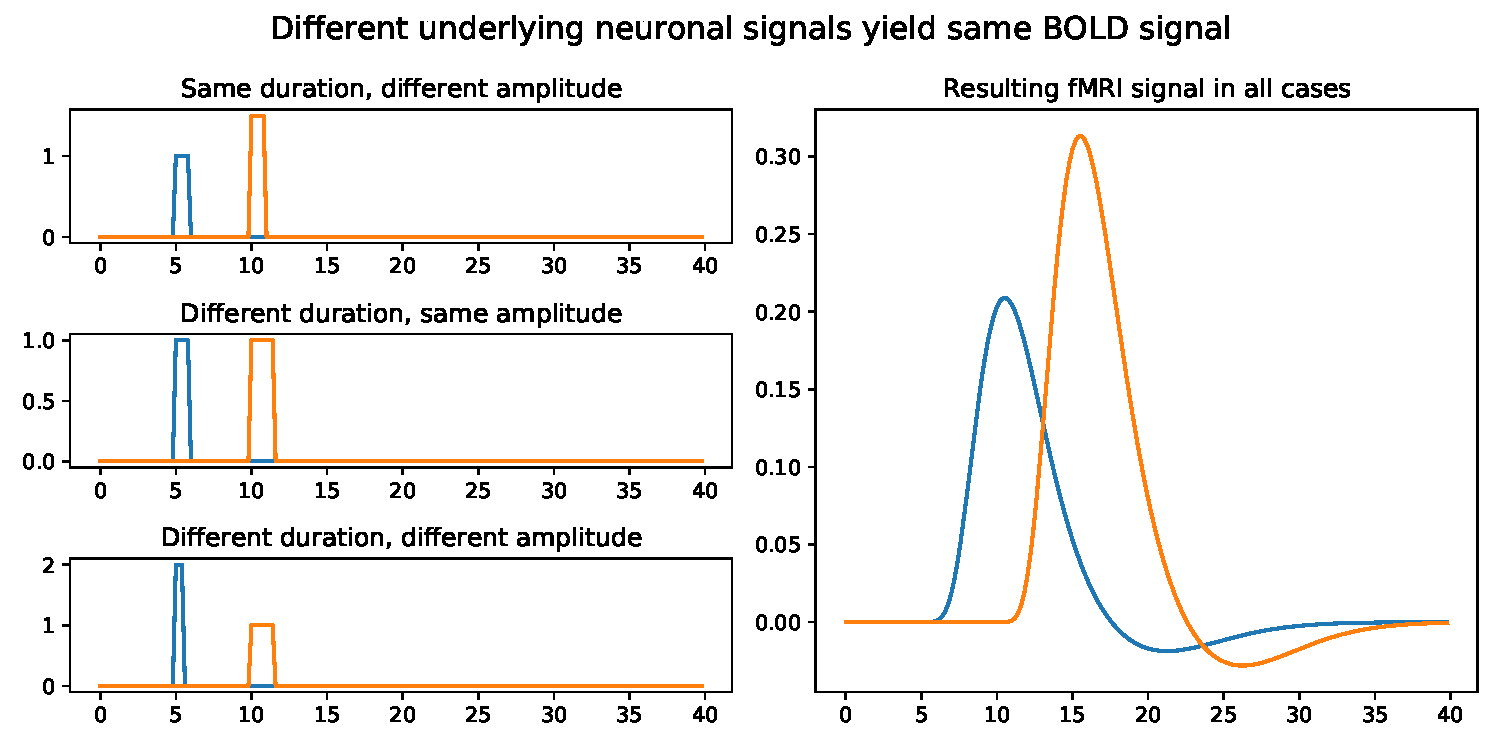
\includegraphics[width=4in]{Figures/neuron_same_bold.pdf}
   \caption{Illustration of how amplitude and duration of neuronal signal interact to yield similar BOLD responses.  The left hand column shows 3 different examples of neuronal signals that evoke the same BOLD response shown in the right hand panel.   }
  \label{fig:neuron_bold}
 \end{figure}

A subsequent series of papers focused on the incongruent versus congruent contrast of the Stroop task and whether activation in the dMFC reflected conflict, as proposed by a prominent theory \citep{botvinick2001}.  This inspiring discourse across multiple publications illustrates the challenge of interpreting RT-based activations as well as demonstrating the rigorous work required to combine the behavioral theory of a task with imaging analysis results when RT-based activation is found.  Both \citet{grinband_dorsal_2011} and \citet{carp_conditional_2010} showed the difference in activation between slow and fast congruent trials was similar to the difference between all congruent and incongruent trials in the dMFC, supporting the idea that the commonly found effect was driven by RTs.   The next step to fully understand this RT-driven effect is the difficult step of determining whether this is a time on task effect or an actual difference in the amplitude of neuronal signaling that correlates with RT and whether these differences align with the underlying theory of conflict in the Stroop task.  This was the focus of follow-up work by \citet{yeung_errors_2011} who proposed that the RT-based effects were a result of differential engagement of specific cognitive processes and not simply due to time on task. They also argued that the result supported the predictions from the computational model that formalizes the conflict monitoring theory.   Even though this series of papers drew attention to how we model and interpret response times in the fMRI based Stroop task, a consensus was not reached \citep{brown_medial_2011, grinbandConflictErrorLikelihood2011,nachevBlindExecutive2011} and it did not have a widespread impact on how the Stroop task is modeled or interpreted in fMRI data. Of the 22 papers published resulting from a PubMed search for ``stroop task fmri 2021'', only 4 addressed RT in their analyses and interpretation of their results.  


It is beyond the scope of the present work to come to an agreement on how to interpret Stroop-based fMRI activation maps that may be driven by RTs, but we use this example to illustrate challenges of modeling RT-based effects in fMRI results and the important implications it can have on theoretical conclusions. If a model only evaluates condition differences, without adjusting for RTs, an observed condition effect has multiple potential interpretations, as the true effect could be: a simple condition difference in the amplitude of neuronal response (not driven by RTs), an RT effect with constant amplitude of the neuronal response (with no condition difference) or a relationship where there is both a condition difference and RT effect. If the result is driven by RTs the question remains as to whether it reflects time on task versus a difference in the amplitude of neuronal signaling. Therefore, our ability to interpret the finding of an unadjusted condition difference, without further analysis and work, is limited at best.

To define some terms that will be used throughout this paper, time series-level analysis refers to linear models of fMRI time series while a group-level analysis refers to an analysis of an estimated fMRI contrast across a set of subjects that could be a single group average (1-sample t-test), group average comparisons (eg. 2-sample t-test), linear associations with a covariate (e.g. phenotype) or other group-level models.   Between-trial RT adjustment is formally carried out in the time series-level. Between-subject RT confounds will only impact group-level models involving group comparisons or associations but not single group averages.  Although we focus on ``2 stage'' models, with only within-subject and group levels, these ideas extend to three stage models where subjects have multiple runs and so analyses are done within-run (time series analysis), within-subject (combining runs) and between-subject.


Limited focus has been given to the link connecting between-trial RT adjustment in the time series analysis to between-subject RT confounds in the group-level analysis. For example, if between-trial RT adjustment is ignored, the incongruent versus congruent Stroop contrast may be  correlated with the within-subject difference in average RT between incongruent and congruent trials.  In earlier work \citep{carpRemovingEffectResponse2012}, this relationship was illustrated by showing that the correlation between age and the contrast estimate of incongruent versus congruent Stroop conditions changes based on whether between-trial RT adjustment is performed. Although this work points out the possibility of between-trial RT adjustment impacting between-subject analyses, the link has not been formally defined.
 
In the present work we extend and improve upon previous attempts to incorporate RT into in fMRI data analysis.   We present a model that separates condition differences, adjusted for RTs, and RT-specific effects.  This model is flexible, obviating the assumption in \citet{grinband_detection_2008} that the duration of the neuronal signal necessarily matches the RTs.  We refer to this type of BOLD signal as ``scaling with RT''.  The RT duration model can bias results when the underlying duration is constant across trials (does not scale with RT).  The model presented here can adapt to either of these situations.  We further quantify the bias in the \citet{grinband_detection_2008} model as well as the most commonly used model that ignores RTs completely.  

We also formally define the relationship between the between-trial RT adjustment, or lack thereof, and potential between-subject RT confounds.  We will show that when between-trial RT adjustment is skipped, the effect size magnitude of these potential between-subject RT confounds is on the order of common effects of interest,  e.g. correlations with various behavioral phenotypes.  Given the substantial interest in brain-behavior relationships in the fMRI literature, this is an important confound to consider.   Although the between-subject confound can be avoided with a proper between-trial adjustment for RT in the time series model, repeating the time series model may be non-trivial in some cases.  For example, when using condition difference estimates supplied in databases for large neuroimaging studies, typically RT adjustment in the times series model is skipped and redoing the time series analysis for thousands of subjects may not be possible for many users of these databases.  Understanding the potential for RT confounds to exist in between-subject analyses is important to consider when interpreting results based on data from these databases.  We propose potential solutions, but they are not guaranteed to work as effectively as repairing the time series analysis.

Finally we replicate and extend the findings of \citet{yarkoni_bold_2009} by demonstrating that the widespread association between RT and fMRI activation is consistent over a set of 7 fMRI tasks, each with approximately 91 subjects.  

The overarching goal of this work is to revive an interest and curiosity in understanding and addressing RT-based confounds to improve our interpretation of fMRI signals and their relationship to underlying theories of RT-based tasks. The suggestions we present are easy to implement and enable the direct estimation of RT-based effects in parallel with condition differences, adjusted for RTs.  This does not limit the researcher, but instead more clearly defines what is being studied, thus providing a cleaner link to underlying behavioral theory and improving the ability of fMRI to help understand brain function.



\section*{Results}

\subsubsection*{Simulations}

The statistical models used for fMRI data generally involve the convolution of a vector representing trial or stimulus onsets with a canonical hemodynamic response function (as shown in Figure \ref{fig:neuron_bold})  to create regressors for use in linear modeling \citep{PoldrackMumfordNichols2009}.  The trials can be represented either as delta functions or as boxcar functions with some duration; when a boxcar is used, it is common to set the duration of the boxcar to a constant value such as the duration of the stimulus, or to some brief default value (such as 0.1 second).  In Figure \ref{fig:models} this model is referred to as ``Constant duration, no RT'' (hereafter as ConstDurNoRT).  Because of the indeterminacy described above, the specific constant value used for stimulus duration will not generally impact the statistical inferences derived from the model, as it will simply scale the values of the parameter estimates along with their variances (assuming the trial durations are relatively short).   This standard approach does not include any information about response times; thus, if two conditions differ in their RTs when the true activation magnitude does not differ, the condition with the longer RTs may have higher estimated activation if the signal scales with RT.  

\begin{figure}
  \centering
   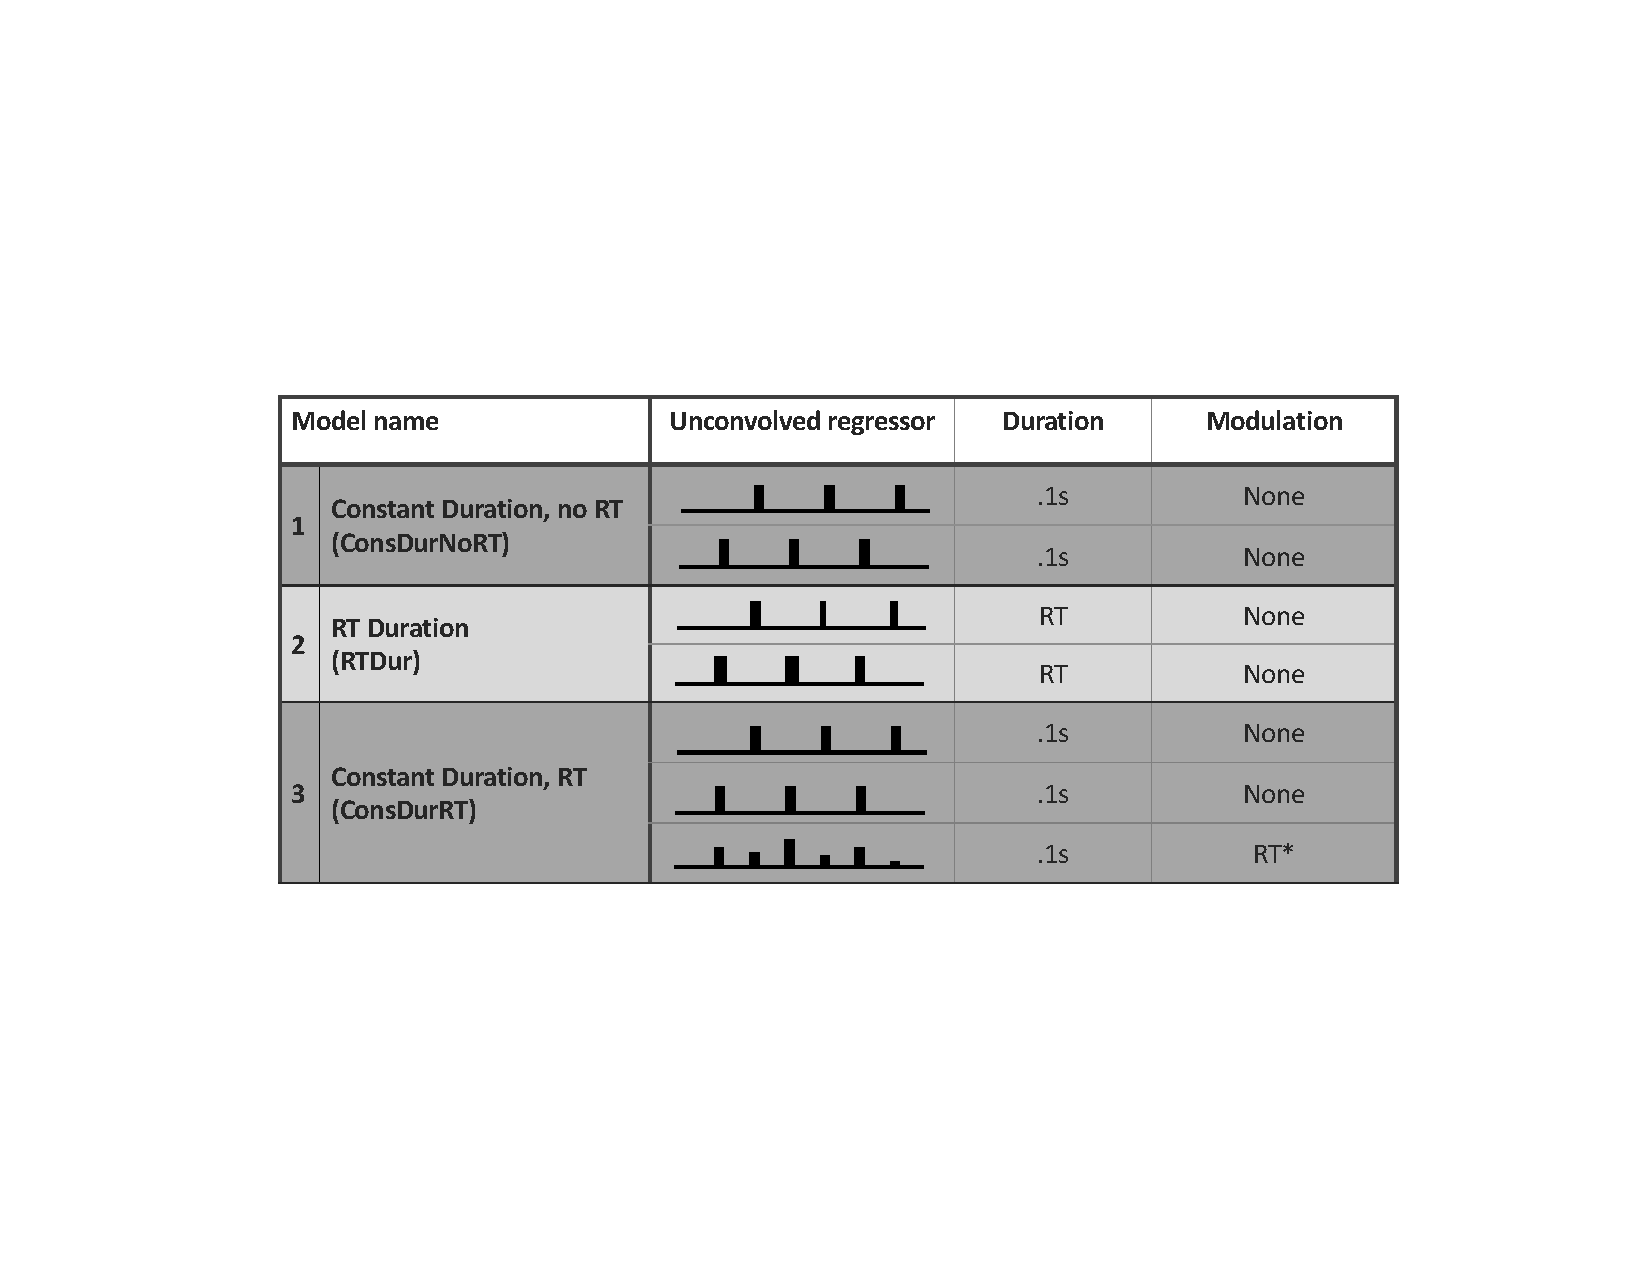
\includegraphics[width=6in]{Figures/model_explainer_new.pdf}
   \caption{Models assessed in the simulation study described by name, unconvolved regressor visualization, duration used for boxcars of unconvolved regressors and definition of the modulation used, when present.  Convolved regressors were used in data generation and modeling.  The first model does not include any response time information, the second model addresses RT through the duration of the regressors and the third model adds an RT modulated regressor to the first model.  $^*$See Discussion for details on why RT is not centered and other details about centering.}
  \label{fig:models}
\end{figure}

\citet{grinband_detection_2008} developed a modeling approach to address the confounding effect of response times in fMRI data, in which the duration of the boxcar function for each trial was varied by the response time on that trial (labeled as ``RT Duration'' in Figure \ref{fig:models} and hereafter as RTDur).  This approach will appropriately scale the parameter estimates for regions in which neural activity duration matches the RT duration, which we will refer to as ``the signal scales with RT''.  Technically, this model implies a restricted condition by RT interaction model, in that it is modeling a separate RT slope, by condition, without main condition effects. Specifically, the model implies each condition has a different linear relationship between BOLD activation and RT, but the intercepts (BOLD activation when RT is 0) are both zero.  Given this, the model has two shortcomings. First, it will not correctly model activation in regions where neural activity does \textit{not} scale with RTs but rather the true duration is an unknown constant across all trials.  Second, it does not allow a separate identification of condition differences versus RT effects; instead, it only performs well if the restricted interaction model is correct.  

To address these issues, we created a generalized model of RT that can identify RT effects separately from the task effect (corrected for RT); this is shown as ``Constant Duration, RT'' in Figure \ref{fig:models} and hereafter as ConstDurRT.  This model includes a boxcar function with constant duration for each of the task conditions, along with a single regressor that models the parametric modulation of the response in relation to RT for each trial. Because all RTs are modeled within a single regressor, any differences in RT between conditions will be removed by this regressor, leaving the condition difference effects to be interpreted as unconfounded estimates of activation in relation to the experimental manipulation. This model can be extended to a full interaction model, if an interaction is suspected, and this will be further described in the Discussion section (``Condition by RT interaction models'') as well as concerns in using an interaction model to study condition differences if there is not a significant interaction present.  We focus on a simpler non-interaction scenario in the simulation studies to illustrate the results of interest and these results nontrivially extend to the interaction model setting.

Notably we have not mean centered RT or subtracted any value from RT on each trial.  This will not have any impact on the estimate of the contrast of interest (condition difference) and would only impact the condition versus baseline contrast estimate in this model.  If RT is mean centered, within run, the interpretation of some contrasts become, ``BOLD activation difference when RT is the mean RT for this run'', necessarily introducing an RT-based confound if this contrast is used as the dependent variable in higher level analyses.  More details about the impact of centering RTs are included in the Discussion (``Should the RT modulation values be centered?''), including examples where it is necessary to center in some way and how to do so without introducing a new confound.  We also discuss why an RT duration regressor is not used instead of the RT modulated regressor. For all models the effect of interest was the subtraction of condition 2 - condition 1, so the RT modulated regressor in ConstDurRT simply serves as a nuisance regressor to pick up RT variability, when present.  Further details regarding the modeling approach can be found in Methods; code and data for all analyses are shared at \textbf{TBD}.

Response time data were simulated based on RTs from two different tasks: the Stroop task (based on a real data analyzed below) and reported RT distribution parameters from a Forced Choice task used by \citet{grinband_detection_2008}.  In each case RTs were generated by sampling from an ex-Gaussian distribution \citep{Ratcliff1976RetrievalPI}; the specified ex-Gaussian parameters led to RTs that were generally longer for the Forced Choice task (mean = 1337, sd = 706.5) compared to the Stroop (mean = 690, sd = 177.5).  Another difference is that the variance relative to the mean is smaller for the Stroop task (coefficient of variation of .528 and .257 for the Forced Choice and Stroop tasks, respectively).   The interstimulus interval (ISI) was sampled from a Uniform distribution. Trials were either randomly presented conditions or blocked conditions, where 4 trials of the same condition were presented in a row.  Time series data that scale with RT were based off of the RTDur regressors and data that did not scale with RT were generated using the ConstDurNoRT regressors. 

All simulation-based results correspond to group level analyses with 100 subjects.  See the Methods for further details on effect size and variance settings.


\subsubsection*{Error rates and power}
 
 We first assessed the false positive rate for each of the models on each of the simulated data sets (Figures \ref{fig:type1err_24}, \ref{fig:type1err_36}). In all cases the ConstDurRT model appropriately controlled Type I error, but error rates were inflated when model assumptions regarding the relationship between RT and neural activity were violated by the data.  Specifically, ConstDurNoRT had highly inflated error rates when activation did scale with RT, and RTDur had inflated error rates when the signal did not  scale with RT.  Thus, the most commonly used model for task fMRI analysis, ConstDurNoRT, suffers from substantial inflation of false positives in the face of RT differences between conditions, because it inaccurately attributes the confounding RT signal to differences in the intensity of the underlying neuronal signal.  The larger Type I error rates observed with the Stroop-based RT reflects that the standard deviation of the RT, relative to the mean, was lower in this setting and so RT-based differences are easier to detect. The error rates for blocked designs (solid lines) are slightly higher, likely due to the fact that blocked designs have a higher signal to noise ratio, making it easier to detect RT differences in the data.  Results with a longer ISI, between 3-6s, are similar (Results shown in Figure \ref{fig:type1err_36}).

\begin{figure}
  \centering
   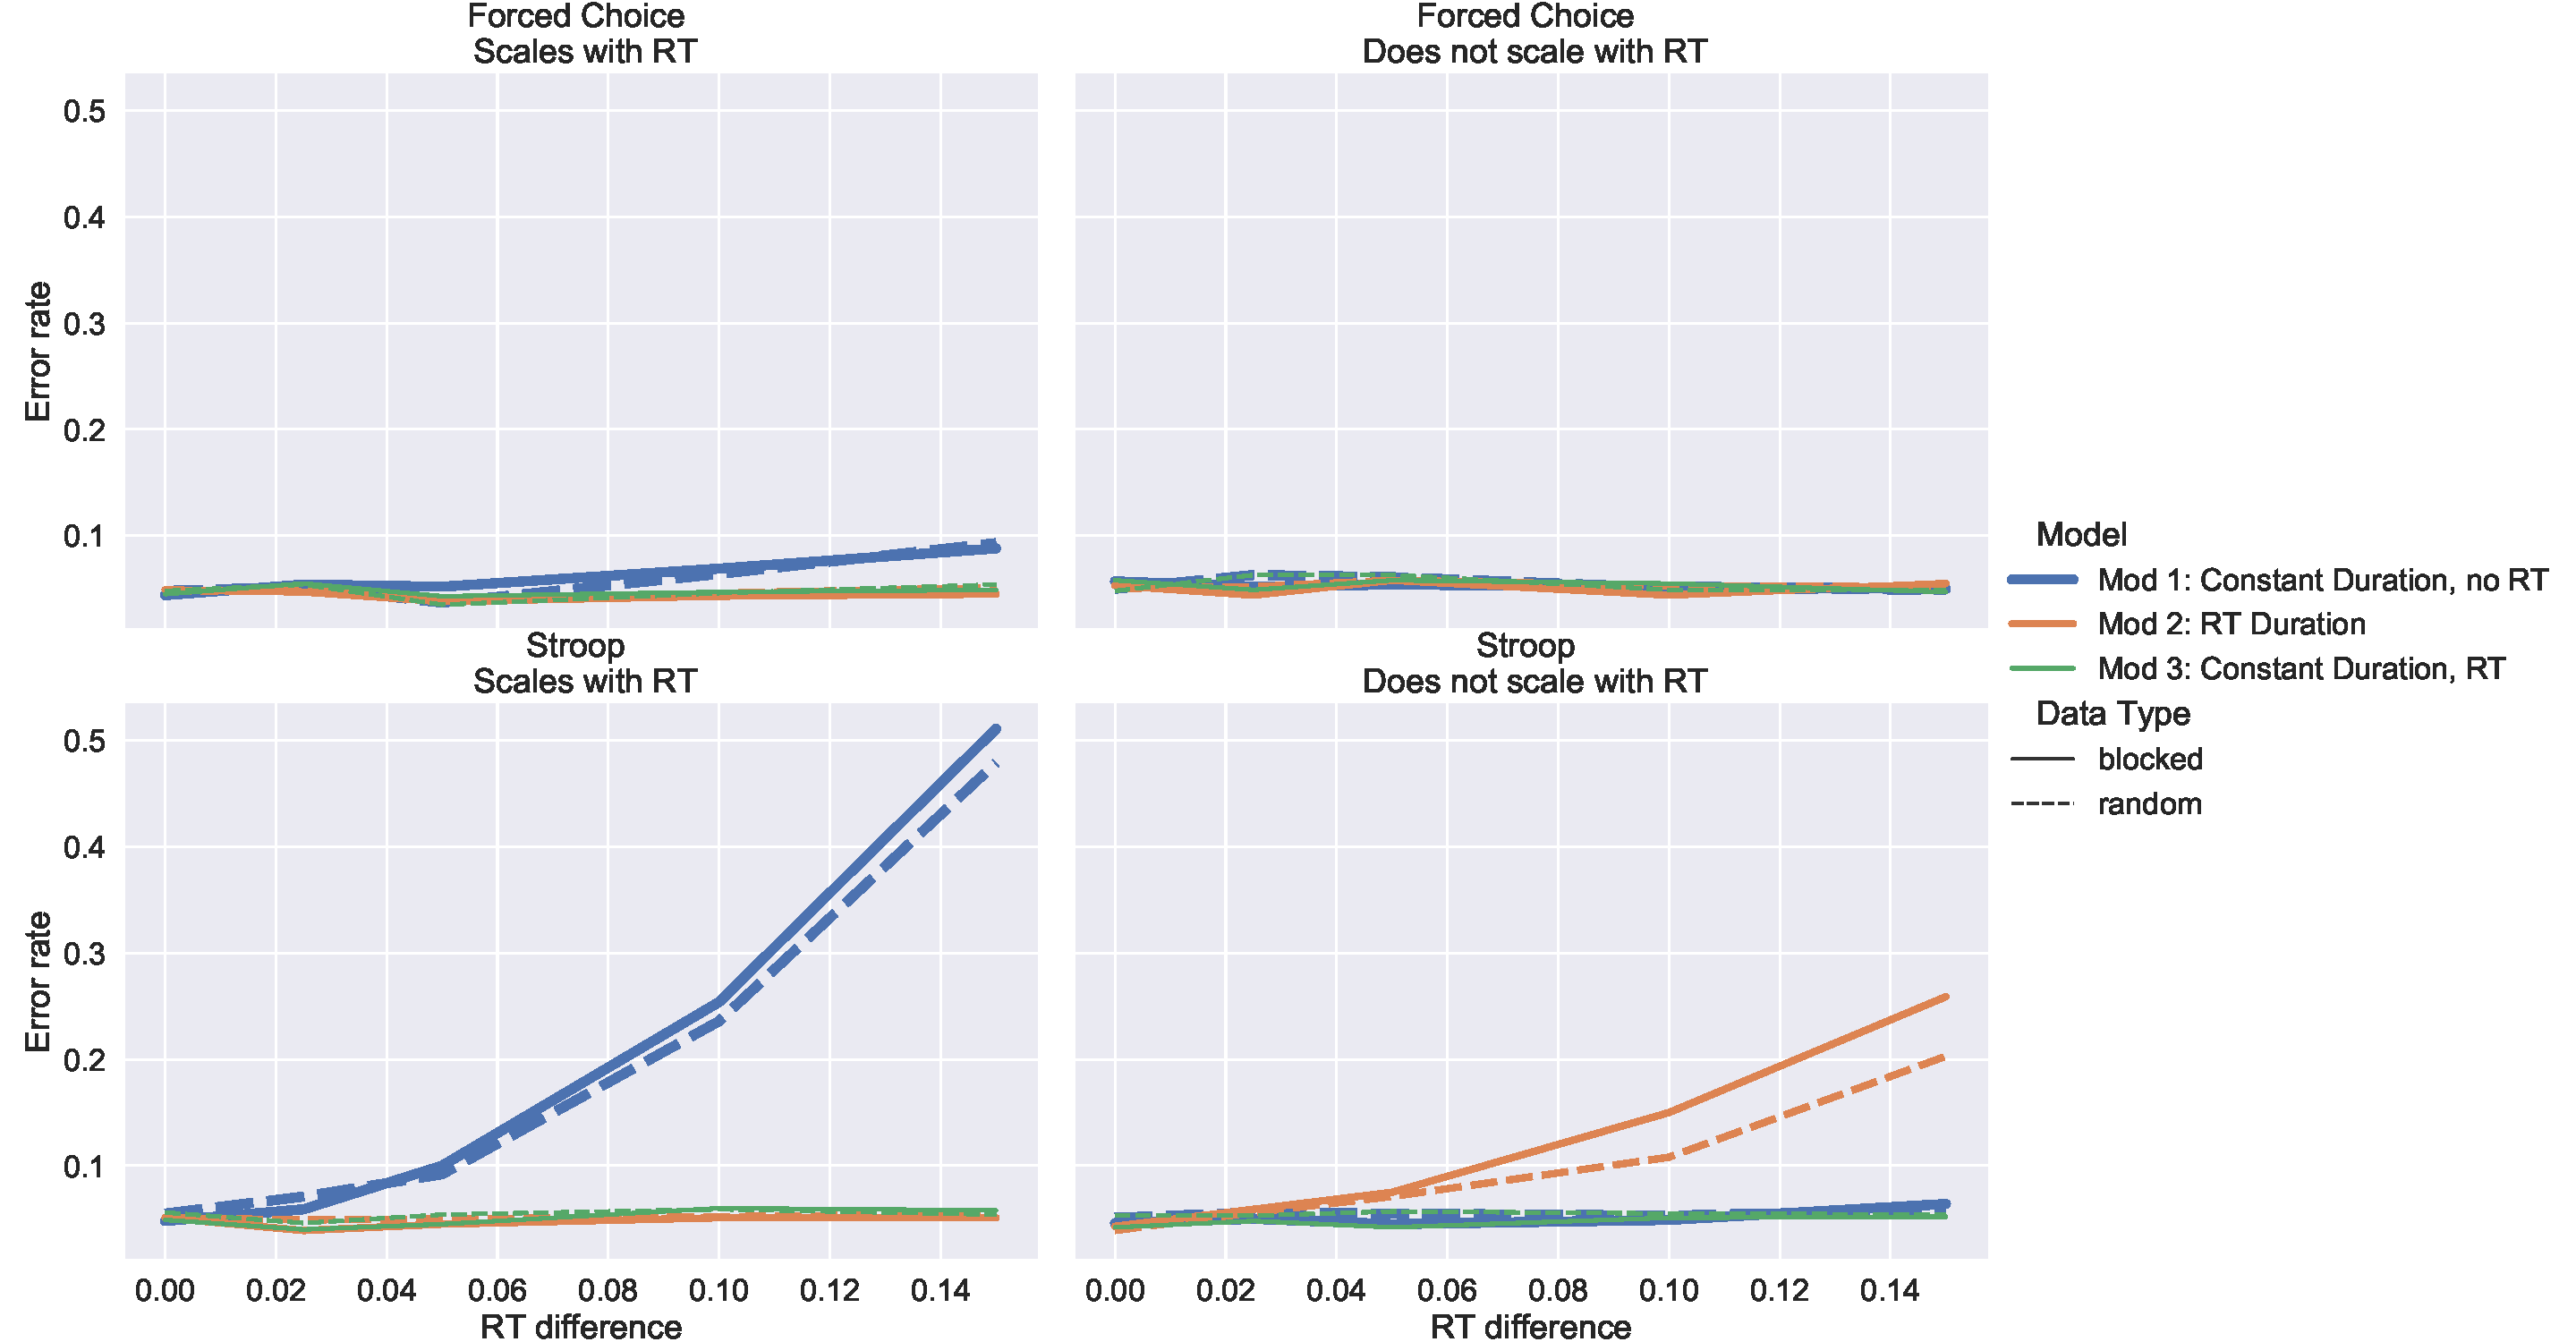
\includegraphics[width=5in]{Figures/type1_err_24.pdf}
   \caption{Type I error as RT difference between conditions increases.  The Forced Choice Task RT distribution was used in the top panels, while Stroop RT distribution was used in the bottom panels, both with an ISI between 2-4s was used and inference of interest was the 1-sample t-test of the condition effect with 100 subjects.  2500 simulations were used to calculate the error rate.}
  \label{fig:type1err_24}
\end{figure}

When signal does not scale with RT power can only be considered for the ConsDurNoRT and ConsDurRT models since the RTDur model did not have controlled error rates. Figure \ref{fig:power_rtdiff}  shows that adding an RT-based regressor, when no RT effect is present, does not impact power at the group level.  Thus the flexibility of the ConsDurRT model to adapt to either the scales with or doesn't scale with RT scenario does not result in a loss in power, which was previously implied in \citet{grinband_detection_2008}, which only studied power at the single subject level and not the group level as done here.  We do not study power in the context of when the signal scales with RT, since the signal generated by scaling each of the RTDur model regressors by different values would represent an interaction model, where the linear relationship between RT and BOLD differs by condition.  In this case the ConsDurRT model is clearly the incorrect model and power is irrelevant.  The more suitable model would fit an interaction effect by replacing the single RT modulated regressor in the ConsDurRT model by condition-specific RT modulated regressors.  Interaction models will be a topic in the Discussion section (``Condition by RT interaction models'').



\begin{figure}[h!]
  \centering
   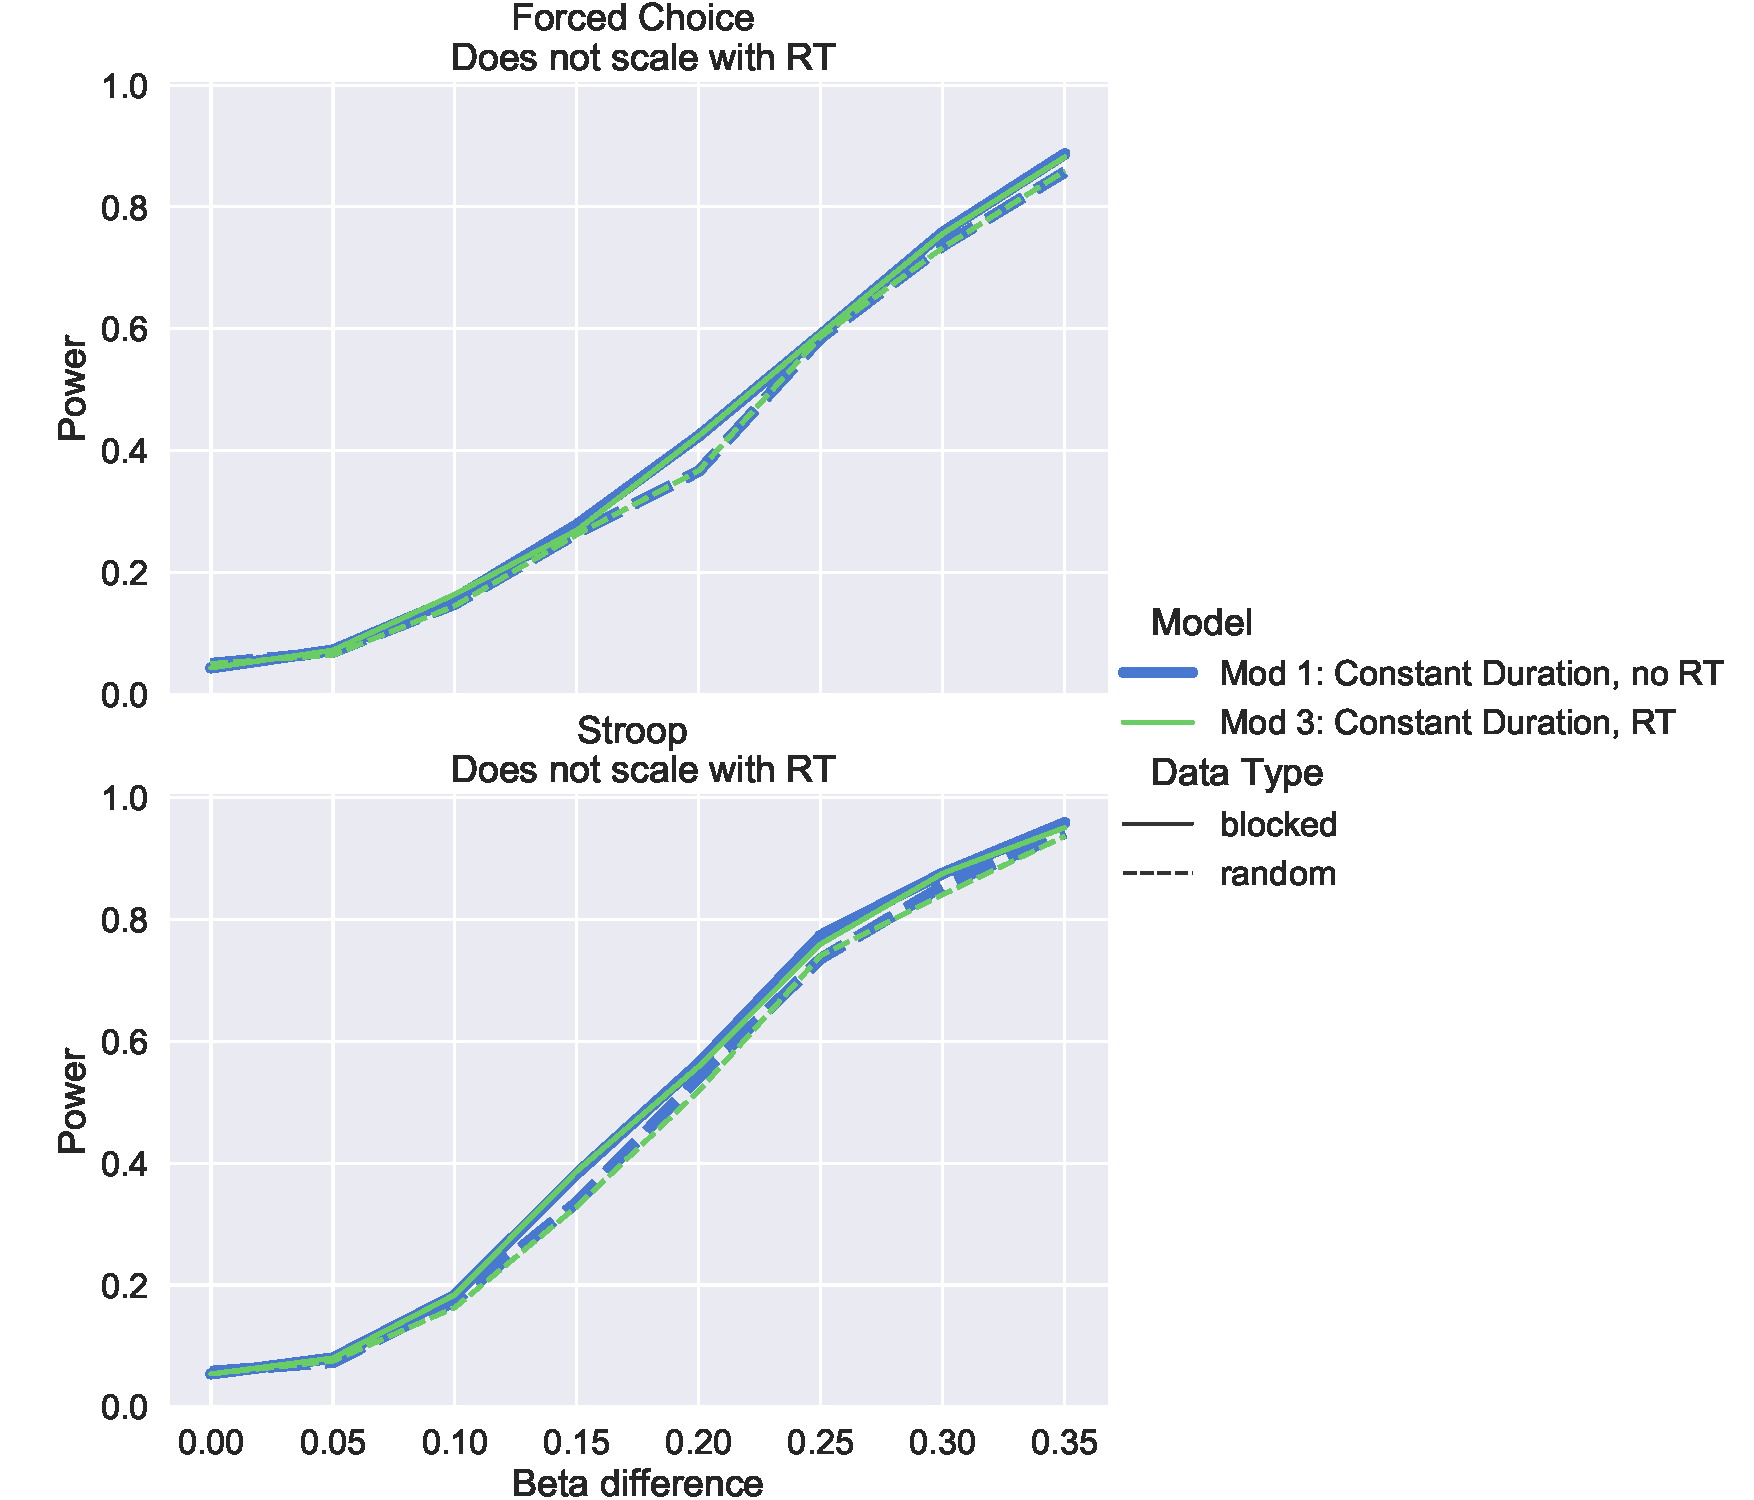
\includegraphics[width=5in]{Figures/power_24_rtdiff_1.pdf}
   \caption{Power when RT difference is 0.1s as the condition difference increases when signal does not scale with RT. The ConsDurRT model (green line) has similar power to the true model, ConsDurNoRT, illustrating no power loss occurs due to including an RT regressor in the time series analysis. Results for RTDur are not shown since it did not have controlled error rates.   Sample size is 100, with an ISI between 2-4s. }
  \label{fig:power_rtdiff}
\end{figure}


\subsection*{RT differences can confound group-level analyses}

The foregoing analyses, along with the previous work by Grinband, focused on confounding of RT between-trials, which impacts average condition effects.  Here we introduce a new problem of a between-\emph{subject} RT confound.  The within-subject differences in average RT, corresponding to the contrasted conditions,  can confound group level analyses involving group comparisons or associations.  For example, the incongruent versus congruent BOLD contrast estimate may correlate with the differences in average RTs for incongruent and congruent conditions.  This is of particular interest given the increasing focus on analyses of brain-behavior correlations in fMRI literature (e.g. \citet{duboisBuildingScienceIndividual2016}).

The driving factor of correlations between condition differences in brain activation and the corresponding differences in RTs is due to a linear relationship between the activation estimate and RT when the data and model assumptions are in conflict. In the case where signals scales with RT and the ConstDurNoRT model is used (duration = 1s), the relationship between the estimated activation, $\hat\beta$, and the true activation, $B$, is approximately $\hat\beta = B \times RT$, for a single trial.  Figure \ref{fig:bold_rt} shows this linear relationship holds within the range of RTs one would expect to observe in most data sets (i.e., $<2$s).  Moving from the activation estimate of a single trial to the BOLD activation across multiple trials, the relationship becomes $\hat\beta = B\times \overline{RT}, $ where $\overline{RT}$ is the average RT across trials.  Last, for two conditions, $1$ and $2$, assuming $B$ is a common true activation, the relationship for the contrast of conditions is $$\hat\beta_1 -\hat\beta_2 = B\times\left(\overline{RT}_1 - \overline{RT}_2\right).$$
From this it directly follows that in a \emph{group} level analysis there is an expected linear relationship between the estimated condition difference and the difference in RTs, specifically the between-subject slope would be $B$, the true, common activation of the two conditions.  As is the case with all linear trends (equivalently, correlations) this relationship does not require a non-zero RT difference on average, but is driven by between-subject RT variability. Therefore the RT difference is an important confound regardless of whether it is significantly different from 0 on average.  

Importantly, in this scenario, although the linear relationship at the group level is simply, $B$, the common activation for both conditions, if the activation differs between conditions or across subjects the confound will potentially be more complex in the between-subject analysis.  Therefore, simply adjusting for RT in a between-subject analysis is not guaranteed to have the same impact as adjustment in the between-trial analysis.

\begin{figure}
  \centering
   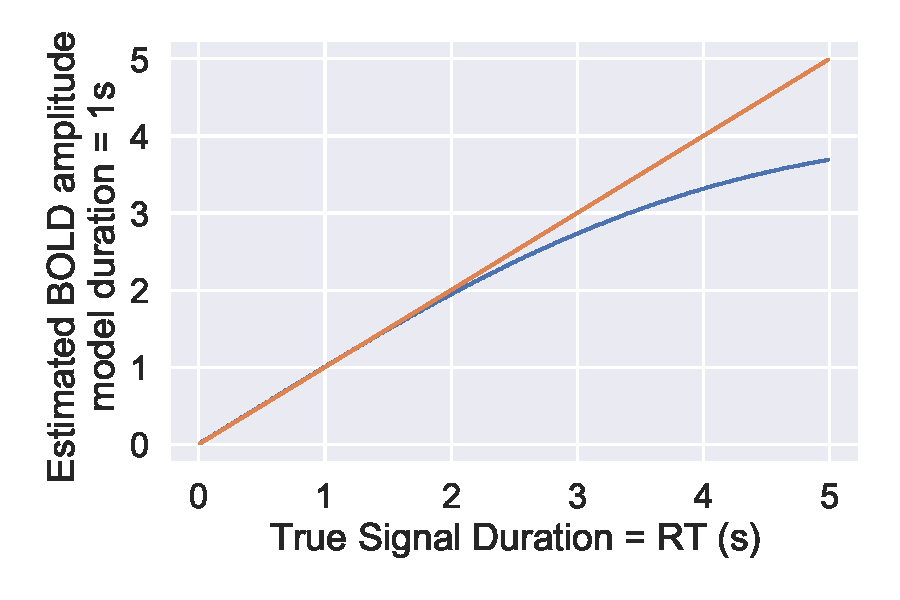
\includegraphics[width=3.5in]{Figures/bold_fcn_rt_1sdur_only.pdf}
   \caption{Relationship between trial RT and the trial-specific BOLD activation estimate when a constant duration of 1s regressor is assumed and signal scales with RT (blue).  Gray dashed line is a line with a slope of 1 and intercept of 0.  The true BOLD activation is 1, but the model estimates the BOLD activation to be $1\times RT$ for RTs $<$ 2s.}
  \label{fig:bold_rt}
\end{figure}


The simulation results in Figure \ref{fig:rt-cor} show the relationship across all models and data types considered in this work. The ConstDurNoRT model produces correlations between contrast differences and RT differences when the signal scales with RT, as does the RTDur model when the signal does not scale with RT while the ConstDurRT model does not induce correlations for either signal type.  Notably, the data were simulated such that the variance in RT did not change with RT, whereas in real data the variance of RT often increases with its mean.  The implication is the correlation estimated by our simulations is conservative.  Even so, it is within the ballpark of the expected true correlations between brain and behavior measures \citep{marekReproducibleBrainwideAssociation2022}.  

Adjusting for the between-subject RT confound within the group level model should only be used when it is not possible to revise the time series analysis to include a between-trial RT confound adjustment, which may be the case when using neuroimaging databases of parameter estimates.  Limitations in this approach should be clearly described when presenting results.


\begin{figure}
  \centering
   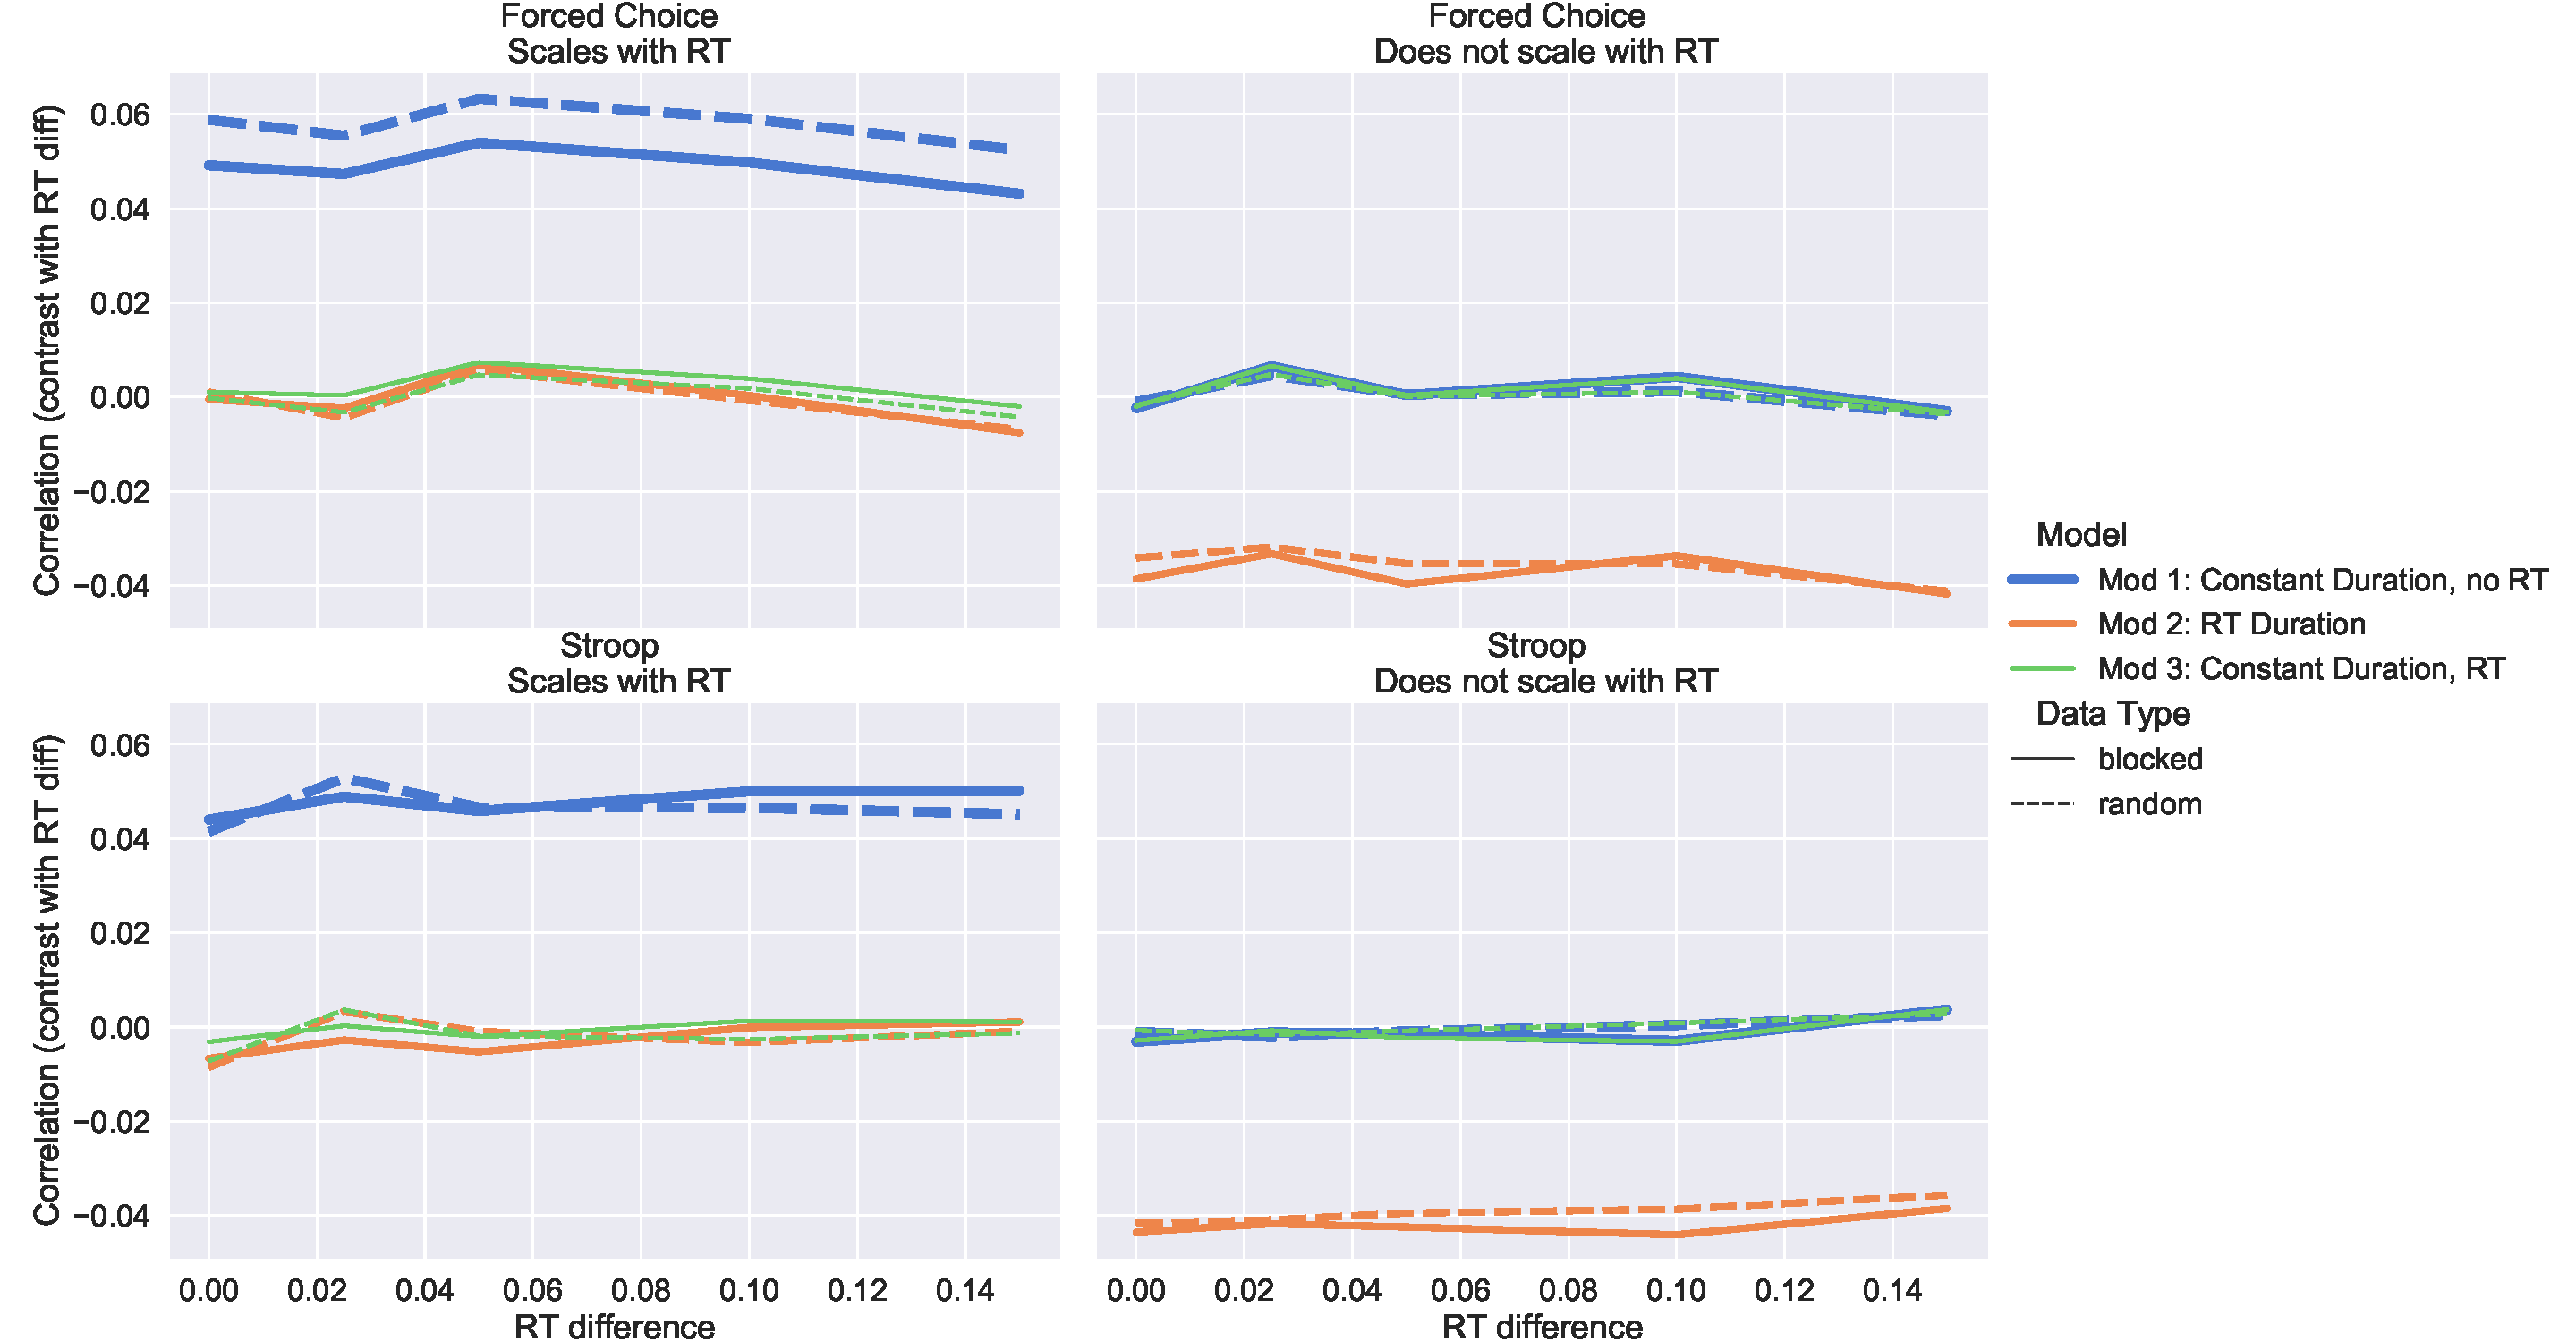
\includegraphics[width=5in]{Figures/cor_with_rt.pdf}
   \caption{Correlation between the contrast difference and difference in average condition RT across subjects as a function of the average difference in RT between conditions.  Since the correlation is driven by between-subject variability in the \emph{difference} in RT, there is no requirement that RTs differ between tasks and the correlation is constant regardless of the RT difference. }
  \label{fig:rt-cor}
\end{figure}




\subsection*{Widespread RT activation is not specific to task, revisited}

Our real data analyses were modeled to included separate regressors for each condition as well as a single RT regressor to control for RT effects in our contrasts between conditions, similar to the ConsDurRT model.  A total of 7 tasks, each with approximately 91 subjects, were analyzed. These tasks putatively capture a broad array of cognitive processes, including attention, temporal discounting, proactive control, reactive control, response inhibition, resisting distraction, and set shifting. Compared to the \citet{yarkoni_bold_2009} tasks, our seven tasks emphasize cognitive control to a greater extent and emotional processing and working memory to a lesser extent. Brief descriptions are given in Table \ref{tab:task_summaries} and more detailed summaries are provided in the Methods section.   The focus here is on the average RT-related effect across subjects.  Notably, this effect estimate will be slightly diminished from a full RT effect, since it is adjusted for condition difference and so the interpretation would be the average within-condition RT effect. Group statistics maps were thresholded using the TFCE p-value (from FSL Randomise) less than 0.05 with 5000 permutations.  The conjunction in Figure \ref{fig:conj} shows voxels where the RT-modulated effects were significant across all 7 tasks.  This is an updated version of the maps shown in \citet{yarkoni_bold_2009}, which used tasks including  3-back, decision making, emotion ratings and memory in sample sizes of 50, 102, 26, 35 and 39.  Our maps are consistent with those, but with a more spatially widespread effects, which may reflect the fact that our sample sizes were larger. In particular, the present comparison demonstrated substantially more signal in the lateral superior parietal cortex.

\begin{table}[h!]
  \begin{center}
    \begin{tabular}{|L{6cm}|L{7cm}|L{1cm}|}\hline
   \textbf{Name} & \textbf{Description} & \textbf{N} \\ \hline\hline
   Attention Network Test (ANT) &  Tests three aspects of attention or  "attentional networks": alerting, orienting, and executive control & 91 \\ \hline
    Delay-Discounting Task (DDT) & Measure of temporal discounting, the tendency for people to prefer immediate monetary rewards over delayed rewards & 86 \\ \hline
   Dot Pattern Expectancy (DPX) & Measure of individual differences in cognitive control including proactive and reactive control modes & 91 \\ \hline
   Motor Selective Stop Signal & Measures the ability to engage response inhibition selectively to specific responses & 91 \\ \hline
   Stop-Signal Task & Measure of response inhibition & 91 \\ \hline
   Stroop & Measure of cognitive control perhaps including resisting distraction or attentional filtering & 94 \\ \hline
   Cued Task-Switching Task (CTS) & Indexes the processes involved in reconfiguring the cognitive system to support a new task & 94 \\ \hline
    \end{tabular}
    \caption{fMRI task summaries}
    \label{tab:task_summaries}
   \end{center}
 \end{table}

\begin{figure}
  \centering
   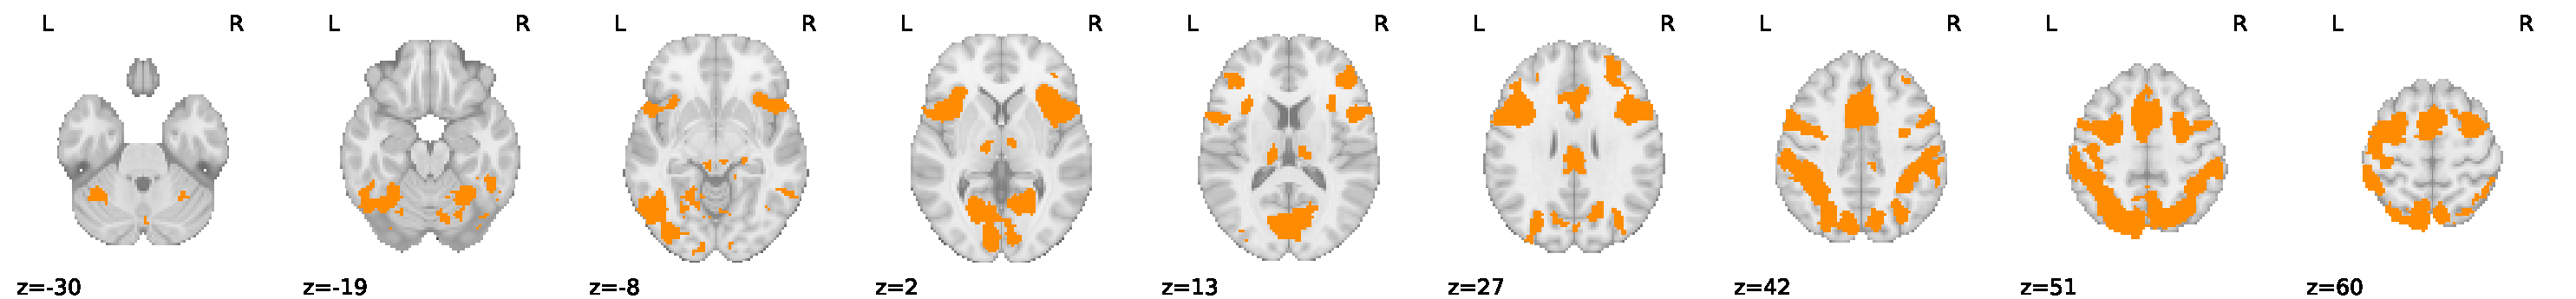
\includegraphics[width=6.5in]{Figures/conjunction_avg_rt_effect_across_7tasks.pdf}
   \caption{Conjunction of the average, within-condition RT effect across ANT, DDT, DPX, motor selective stop, stop signal, stroop, and CTS.  On average, each analysis included around 91 subjects and maps were corrected for multiple comparisons using a TFCE p-value thresholded at 0.05 using 5000 permutations.}
  \label{fig:conj}
\end{figure}


%\begin{figure}
%  \centering
%   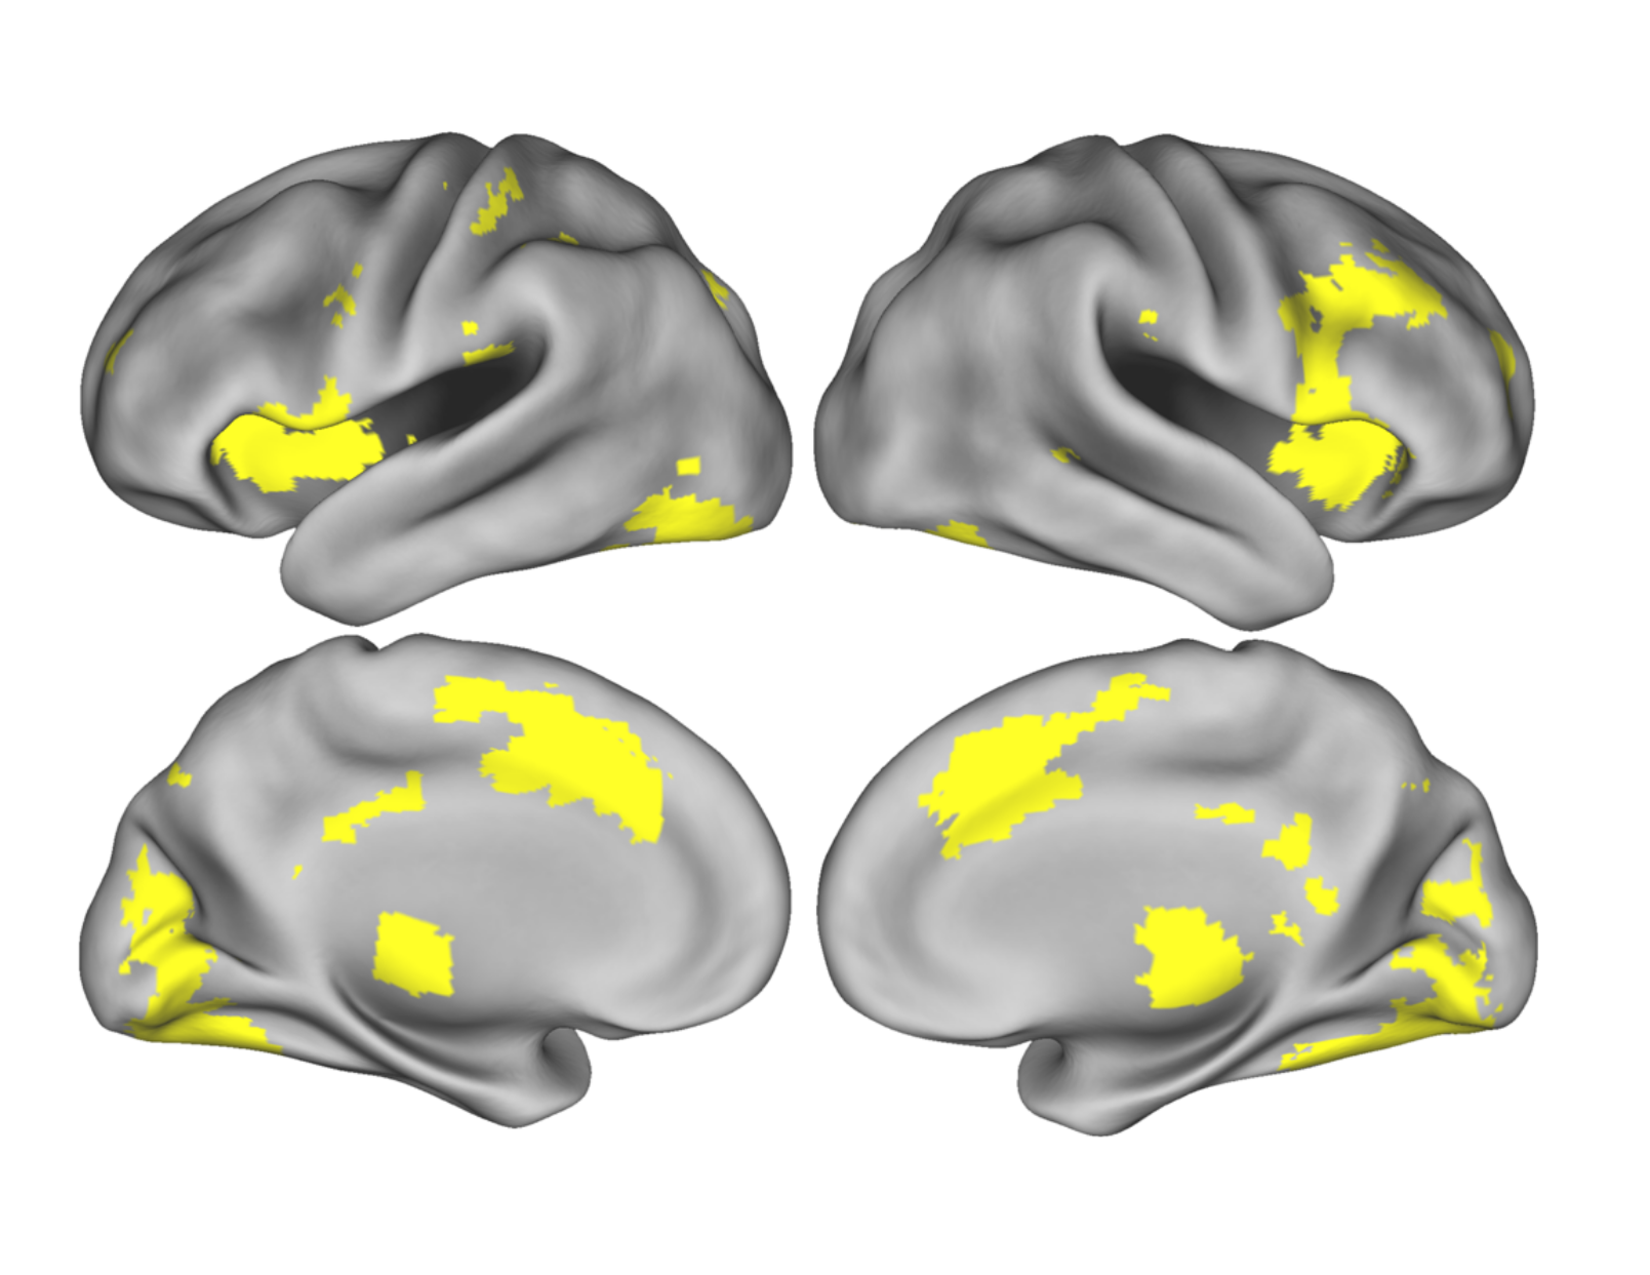
\includegraphics[width=4in]{Figures/temporary_fig_from_yarkoni.pdf}
%   \caption{TEMPORARY.  This is the figure from Yarkoni for comparison during revisions. From that paper: Figure 2. Cortical regions that showed significant RT-related activation in all five samples. Clockwise from top left: ,left lateral, right lateral, left medial, and right medial views of the cortical surface. doi:10.1371/journal.pone.0004257.g002}
%  \label{fig:conj-yarkoni}
%\end{figure}


\section*{Discussion}

The problem of potential response time confounds for fMRI activation estimates has been discussed for more than a decade, but there has been little resulting change in how the community approaches the analysis and interpretation of fMRI contrasts when RT differences between task conditions are present.  There are three takeaways from the present work.  First, we propose a modeling approach that more effectively adjusts within-subject contrast estimates for response time differences, so that group average estimates of contrasts are adjusted for between-condition response time differences.  Second, this work highlights an important problem that has not been discussed previously: 
the presence of a between-subject analysis confound of the average RT differences.  Finally, we replicate previous work showing that RT-related effects are not task specific \citep{yarkoni_bold_2009}.

This work presents a model that can adapt to data whether or not the signal scales with RT, without losing performance. By adding an RT modulated regressor to the most commonly used model that only contains condition-specific regressors, the ConstDurRT model reduces RT-driven type I errors in average condition comparison effects without a reduction in power.  The commonly used ConstDurNoRT model assumes the signal does not scale with RT and the RTDur model assumes the signal must scale with RT, hence both models fail to control error rates when these model assumptions are violated (Figure \ref{fig:type1err_24}).  


We have also uncovered that subject-specific differences in average RT represent an important group-level confound.  This confound is only present if the time series model follows the ConsDurNoRT or RTDur approaches, whereas the ConsDurRT model produces condition difference effects that are free of this confound.  Notably, the average difference in RT across subjects does not impact the strength of the correlation, since the correlation is driven by the variability in RT differences across subjects.  Thus, even if the RT difference is 0, the first level models should include a between-trial RT adjustment.  If it is not feasible to repeat the first level analyses, which may be the case for users of large neuroimaging databases of activation estimates, there are limitations to simply adjusting for RTs at the group level. Group level RT adjustment will only succeed in fully removing this confound if the activation magnitude is equal across conditions and subjects.


Last, our updated RT-effect conjunction analysis across 7 tasks tapping into different mental processes show widespread shared activation in the so-called ``task-positive'' network, replicating the previous results of \citet{yarkoni_bold_2009}. This highlights the generality of the RT effect across tasks, and motivates the need to model these effects across all tasks.  

\subsection*{The paradox that RT is the effect of interest in fMRI studies}

Our recommendation here is to focus separately on RT-based effects and condition differences, adjusted for RT.  There can be resistance to this idea, since RT is the measure of interest in behavioral studies and removing RT effects from condition differences is argued to be ``throwing the baby out with the bathwater''.  This argument is paradoxical since if RT effects are the effects of interest, then why not study the RT effects directly? Studying unadjusted condition differences does not directly reflect RT effects and may reflect differences that are completely unrelated to RTs.  In fact the condition difference effect, when unadjusted for RTs, may be driven by any of the underlying models shown in Figure \ref{fig:underlying-theory} and this fact should be made clear when presenting any results based on the ConsDurNoRT model.  If the RT based effect is the effect of interest, it should be studied directly using a model that mirrors the underlying theoretical model of RTs relationship with the construct of interest to maximize power.  A significant finding is just the beginning and further work is necessary to establish whether the RT-based effect reflects time on task or an amplitude-driven effect, as was argued for the Stroop task by \citet{yeung_errors_2011}.  If this important extra work is not done, then conclusions for unadjusted RT effects must be presented acknowledging the limitations in their interpretation.

Overall our recommendation of focusing on RT-based effects and condition differences, adjusted for RTs, doesn't throw anything away, but separates two effects so they can be more accurately interpreted, ultimately improving our understanding of the brain. 

\begin{figure}
  \centering
   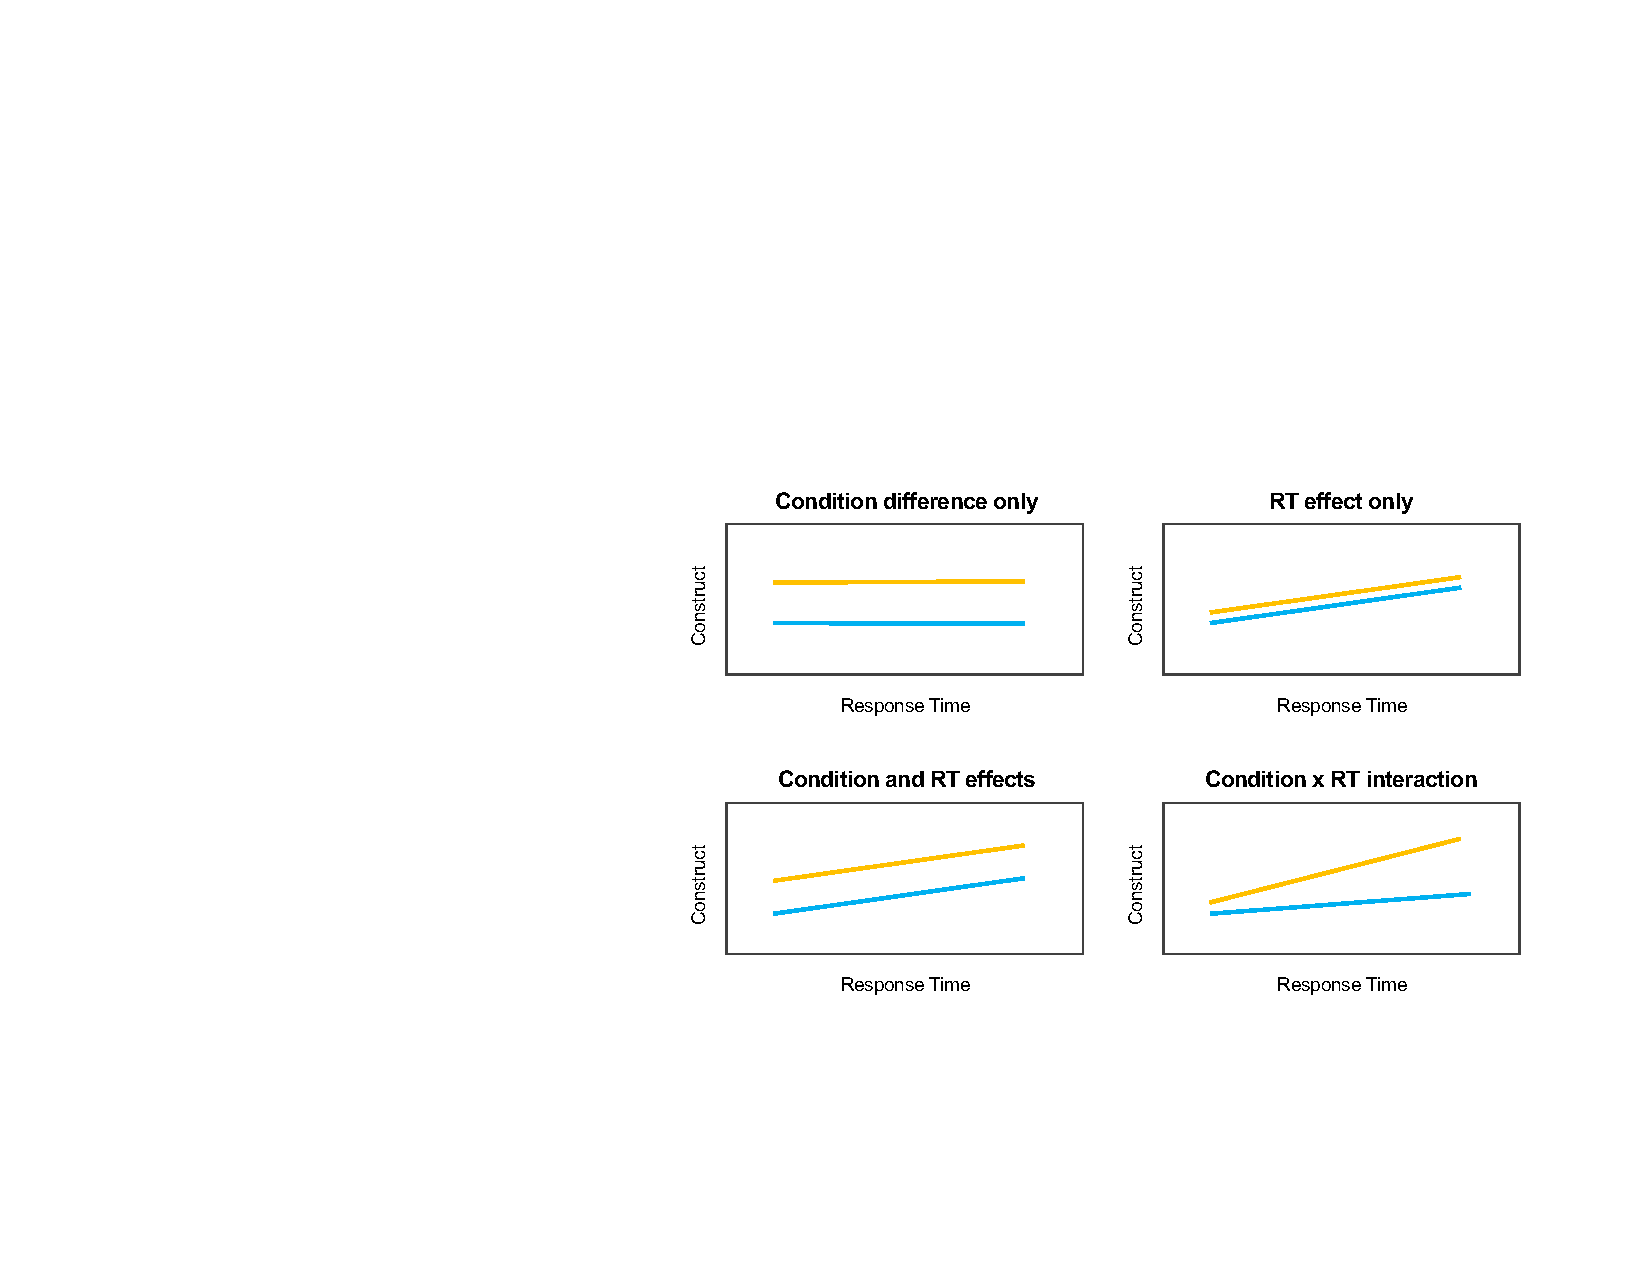
\includegraphics[width=4in]{Figures/underlying_theory_models.pdf}
   \caption{The ConsDurNoRT model assumes the underlying relationship between the construct of interest follows the ``Condition difference only'' model.  Since the condition difference model can yield significant results when \emph{any} of these models is the true underlying model, only nonspecific interpretations can be made from the ConsDurNoRT model results.  To strongly link brain activation to a specific construct of interest, the fMRI model should mirror the underlying behavioral theoretical model.}
  \label{fig:underlying-theory}
\end{figure}

\subsection*{Modeling considerations}

\subsubsection*{Should the RT modulation values be centered?}
We did not center RT in our models, as it would not have any impact on the condition difference estimate since trials in both conditions involve RTs and the model implies the same condition difference effect occurs for all RTs.  A common practice is to center by the mean RT for that subject and run of data, but this can introduce RT information into some contrast estimates.  For example, if RT is centered, the interpretation of a condition versus baseline effect is specifically for that subject/run's mean RT.  In this case there is an RT confound introduced at the group level since each subject's activation reflects their own RT.  The same will occur for any contrast where one condition involves RTs and another does not.  For example, in the stop signal task the go trials have a response time whereas successful stop trials do not.  Therefore if RT is centered within-subject and run, the go versus successful stop contrast estimate corresponds to the magnitude of the effect for mean RT of that subject/run, such that a correlation between this contrast and the average go RT will leak into the group level analysis.  A summary of contrast types that are impacted by centering RT is given in Table \ref{tab:centering-rt}.

To avoid this issue simply center by the same value for all subjects and runs.  This value can either be the mean RT across \emph{all} subjects and runs or a value that is roughly what one would expect the average RT to be for that task.  In this case the RT confound at the group level should not be present.  If all condition comparisons involve conditions with RT effects (as is most often the case for contrasts of interest in cognitive fMRI studies), then centering RT in the modulated regressor will have no effect on the contrast estimates of interest.

\begin{table}[h!]
  \begin{center}
%    \begin{tabular}{|L{6cm}|L{7cm}|L{4cm}|}\hline
   \begin{tabular}{|L{4cm}|L{3.25cm}|L{3.9cm}|L{3.7cm}|} \hline
      Contrast type & Example  \newline (stop signal task) & Interpretation without centering RT & RT centering necessary with ConsDurRT model? \\ \hline\hline
      Condition (RTs) vs. baseline & Go  vs. \newline baseline & Go activation when RT is 0 & Yes \\ \hline
      Condition (RTs) vs. Condition (no RTs) & Go vs. \newline  Successful Stop  & Condition difference when Go RT is 0 & Yes \\ \hline
      Condition (RTs) vs. Condition (RTs) & Go vs. \newline  Unsuccessful Stop & Condition difference & No \\ \hline
    \end{tabular}
        \caption{Whether or not centering of the RT modulated regressor is necessary when using ConsDurRT to study adjusted condition differences.  When centering is required do not use the mean RT for the run, but use the same centering value for all subjects and runs to prevent incorporating an RT counfound in between-subject analyses.}\label{tab:centering-rt}
   \end{center}
 \end{table}


\subsubsection*{Why an RT modulation is used instead of RT duration}

It may seem counterintuitive that we model RT through a parametrically modulated regressor in the ConsDurRT model, instead of a single RT duration style regressor.  This is because the RT centering, described in the previous section, is a special type of orthogonalization that is not possible to carry out directly with the RT duration style regressors.  Generally the RT modulated regressor is a very close approximation to the RT duration regressor, so it is an excellent substitute with more flexibility so we can properly adjust it to improve the interpretation of condition difference contrasts without introducing a new between-subject RT confound.  


\subsubsection*{Avoiding common pitfalls when adding RT to a time series model}
When adding RT to the time series model, there are some  common mistakes that should be avoided.  Most of the problem relates to the intuition that collinearity between regressors is problematic and thus that mean centering or orthogonalization is always necessary.  Once the data have been collected, collinearity with regressors of interest often cannot be resolved, but may have been preventable with a different study design.  If the RT regressor is highly collinear with the task contrast, this should not be altered by orthogonalization or centering RT within task, as that is in conflict with the motivation for adding RT in the first place: controlling condition differences for RT differences or time on task effects.  If RT is mean centered within-condition, then it is misleading and incorrect to claim the condition effects have been adjusted for RT differences.  If RT is split into separate regressors by condition, this model implies an interaction effect between condition and task is suspected.  In this case, if the interaction is significant, then that is the contrast to be studied in detail as it indicates the magnitude of the condition difference varies by  RT.  One should not use an interaction model to study main condition effects, even if the interaction is not found to be significant, which is discussed in the next section.  Our recommendation is if there is not an expected interaction between different conditions and RT, then a single RT regressor should be used.  


\subsubsection*{Condition by RT interaction models}

If the underlying theory about the relationship between the psychological measure of interest and RT implies a condition by RT interaction, then an interaction model should be used in the fMRI analysis.  Specifically the single RT regressor from ConsDurRT would be split by condition and no RT centering should be applied.  In this case the effect of interest is the difference in the RT modulated regressors for each condition.  If the interaction is not found to be significant, we discourage using the interaction model to then study the main condition effects, as recommended in \citet{carp_conditional_2010}.  Although finding the interaction is not significant implies the true slopes between RT and BOLD activation are not different between conditions, the estimated slopes will be different and this adds noise into the condition difference estimate, which reduces power.  Instead, to study main condition differences when the interaction is not found to be significant, we recommend simplifying to the ConsDurRT model.  A group level power analysis (Figure \ref{fig:pow-int}) indicates that the additional noise introduced when using the interaction model results in a loss in power as high as 9.5\% compared to the ConsDurRT model (Figure \ref{fig:pow-int}).  Of course, to avoid inflated error rates, p-value thresholds should use a correction for mulitple comparisons (e.g. Bonferroni correction) to correct for testing both the interaction and then the main condition effect if the interaction is not found to be significant.

\subsubsection*{How to adjust for the RT confound in group level analyses}

To avoid RT confounds in group level analyses, we recommend including between-trial RT adjustment.  If it is not possible to repeat the first level analyses with this adjustment, then a limited approach can be used to attempt to remove RT confounds in the group level model.  The contrasts used in the simulations above were simple differences between two conditions, but other contrasts may be more complex.  A general, flexible approach for removing RT confounds in higher level analyses, is to  add a single average RT regressor for \emph{each} condition involved in the contrast in the group level model.  For example, if positive, negative and neutral conditions for a task were combined in a contrast estimate at the time series level, one would add three RT regressors to the higher level analysis: the mean RT for each of positive, negative and neutral trials.  This will provide limited RT adjustments for coefficients for slopes (correlations) and also contrasts comparing groups.  Importantly, results should clearly explain the limitations in this approach and that an RT-based confound may still be impacting results. This adjustment will only work well if the BOLD activation is equal across conditions and subjects, which is unlikely.

Notably, no RT adjustment at the group level can repair group averages. For example, the group average incongruent versus congruent effect cannot be corrected for RT differences at the group level. The RT adjusting procedure described here only partially adjusts for RT confounds in analyses of slopes and group differences, but not single group means. This is a limitation when using effect size estimates from neuroimaging databases. The interpretation of any average group effects found must account for the possibility that the effect is driven by time on task, as reflected by the inflated error rates in Figures \ref{fig:type1err_24}, \ref{fig:type1err_36}.

 


\subsection*{Limitations of this work}
The primary limitation of this study is that it is simulation-based, which required specififying a large number of parameters including the RT distribution for each condition, effect size for each condition, stimulus length, ISI,  within-subject variance and between-subject variance.  In an effort to set these parameters to realistic values we focused on the size of the within-subject condition effect, aiming for correlations 0.07-0.08, ratio of total variance to within-subject variance, $\frac{SD_{total}}{SD_{within}}$,  ranged between 2-3 and the Cohen's D for the average of task versus baseline across subjects was approximately 0.85.  Higher between-subject variance (lower $\frac{SD_{total}}{SD_{within}}$) would yield smaller time on task effects.  Additionally we only shifted the mean parameters of the Exponential Guassian distributions used to define the RT differences between conditions, whereas our analysis of our own Stroop data showed the variance increased with average within-subject RT.  This increased variance would only strengthen the between-subject correlation between the condition contrast and RT difference at the group level.   Even though these limitations exist, we believe our results to be accurate representations of the RT effect based on consistencies with other studies focusing on the RT effect \citep{yarkoni_bold_2009, brown_medial_2011, grinband_dorsal_2011}.  %In addition, the findings of \citet{li_neural_2021} using 949 subjects from the Human Connectome Project data set, the authors modeled 2-back versus 0-back, without RT adjustment.  Although time on task effects were not the goal of that analysis, their results show that the patterns of activation for the 2-back vs 0-back comparison was very similar to the correlation of the 2-back vs 0-back contrast with the average RT difference between 2-back and 0-back, paralleling our findings indicating RT is an important confound at the group level.  \textbf{this last sentence is a bit unwieldy...}



%\subsection*{Conclusions}

%The interpretation of task fMRI data is fundamentally limited by the presence of a paradoxical confound: The response time differences that are of primary interest to the experimental psychologist reflect a confound in the context of fMRI analysis, due to the slow nature of the hemodynamic response which makes it impossible to distinguish between differences in intensity versus duration of the neuronal response.  This problem has been understood for more than a decade, yet has largely not been addressed in most task fMRI studies.  We propose that the effective use of task fMRI to understand the brain will require the field to come to terms with this paradox.

\section*{Methods}

\subsection*{Models considered}

\subsubsection*{Data generation and modeling} 


The interstimulus interval (ISI) was sampled from a Uniform distribution and RT was sampled from an ex-Gaussian distribution.  For RT, a subject specific $\mu_{sub}$ was obtained by sampling an ex-Gaussian with parameters $\mu_{rt}$, $\sigma_{rt}$ and $1/\lambda_{rt}$ and subtracting the sampled value by $1/\lambda_{rt}$.  The subject-specific RTs were then sampled from an ex-Gaussian distribution with $\mu_{sub}$, $\sigma_{rt}$ and $1/\lambda_{rt}$.  
When RT differed between conditions, each Condition 1's RT mean was $\mu_{sub} - \Delta RT/2$ and Condition 2's was $\mu_{sub}+\Delta RT/2$, where $\Delta RT$ was the RT difference.  Values of $\mu_{rt}$, $\sigma_{rt}$ and $\lambda_{rt}$ were based on our Stroop data and the Forced Choice Task in \citet{grinband_detection_2008}.  In both cases distributions were fit to subject-specific data and then parameters were averaged over subjects.  The Forced Choice RT distribution was defined by a Gamma distribution with shape parameter = 1.7, beta = 0.49.  Sampling from this distribution and fitting an ex-Gaussian to that sample resulted in ex-Gaussian parameters of $\mu_{rt} = 638$, $\sigma_{rt} = 103$, and $1/\lambda_{rt} = 699$ (mean = 1337, sd = 706.5). The Stroop data had faster RTs with less variability, with ex-Gaussian parameters of  $\mu_{rt} =530$, $\sigma_{rt} = 77$, and $1/\lambda_{rt} = 160$ (mean = 690, sd = 177.5).  The distribution functions from Python's Scipy module were used to simulate and estimate the distribution parameters. Trials were either randomly presented conditions or blocked conditions, where 4 trials of the same condition were presented in a row.
 


Simulated data that scaled with RT were created with the convolved RT duration regressors (RTDur) and data that did not scale with RT used the constant duration regressors (ConsDurNoRT).  The BOLD activation sizes for the $i^{th}$ subject for each condition, $\beta_{i, 1}$ and $\beta_{i,2}$, were  sampled from a Gaussian distribution, $N(\beta, \sigma_b^2)$,  where $\beta$ is the true activation magnitude and $\sigma^2_b$ is the between-subject variance.  The time series data for the $i^{th}$ subject, of length $T$, was created according to 
\begin{equation} \label{eq:timeseries}
   \vb{Y_i} = \vb{X}_{1}\beta_{i, 1}  +  \vb{X}_{2}\beta_{i, 2} + \epsilon, \hspace{.1in} \epsilon \sim N(0, \sigma^2_w), 
\end{equation}
where $\vb{X}_{1}$ and $\vb{X}_{2}$  are either the Model 1 or 2 regressors $(T\times 1)$  and $\sigma^2_w$ is the within-subject variance.  


In an effort to choose realistic values for $\beta_1$, $\beta_2$, $\sigma^2_w$ and $\sigma^2_b$, we considered the first level effect size (converting the true $\beta_j$ to a  correlation), second level effect size for a 1-sample t-test (Cohen's D) as well as the ratio of the total mixed effects variance to the within-subject variance.  Following the definitions of parameters as given in the model above, the total mixed effects variance for a first level contrast of parameter estimates is
\begin{equation} \label{eq:mfxvar}
 \sigma^2_{mfx} =  \vb{c}(\vb{X}'\vb{X})^{-1}\vb{c}'\sigma^2_{w} +\vb{c}\vb{c}'\sigma^2_b,
\end{equation}
where $\vb{X}$ and $\vb{c}$ are the first level design matrix (based on models in Figure \ref{fig:models}) and contrast of interest \citep{mumford_modeling_2006}.  The contrast of interest for each model corresponded to condition 2 $>$ condition 1 ($\vb{c}=[-1,1]$ for the 2 regressor models and $\vb{c}=[-1,1, 0]$ for the three regressor model).  The ratio of total SD to within-subject SD is defined by
\begin{equation}\label{eq:sd_ratio}
\frac{SD_{total}}{SD_{within}} = \frac{\sqrt{\vb{c}(\vb{X}'\vb{X})^{-1}\vb{c}'\sigma^2_{w} + cc'\sigma^2_b}} {\sqrt{\vb{c}(\vb{X}'\vb{X})^{-1}\vb{c}'\sigma^2_{w}}},
\end{equation}

Our within-subject effect size for condition versus baseline was between 0.07-0.08 (correlation), ratio of total variance to within-subject variance, $\frac{SD_{total}}{SD_{within}}$,  ranged between 2-3 and the Cohen's D for the average of task versus baseline across subjects was approximately 0.85.

Each run contained 40 trials of each condition and a time resolution (TR) of 1s.  Time course length varied, as it was set to extend 50s past the last stimulus offset.  Group analyses included 100 subjects.  A total of 1000 data sets were simulated to calculate power and error rates. 


Regressors were constructed by convolving boxcar functions with a Double Gamma hemodynamic response function (HRF) using the \verb+compute_regressor+ function from the Nilearn module in Python.  

Least squares regression was used to estimate the models described in Figure \ref{fig:models} at the first level including a set of cosine basis functions (0.1 Hz cutoff) for highpass filtering generated with the \verb+cosine_drift+ function from Nilearn in Python.  At the group level, 1-sample t-tests were used to assess type I error and power.  A correlation of the average difference in RT between conditions and the fMRI contrast (condition 2 vs condition 1) was estimated for each group analysis.  

Since RT and ISI values are random, the contribution of the design matrix, $X$, to the overall variance varies between samples (Equation \ref{eq:mfxvar}) and the true effect size was variable.  Therefore, to calculate the first level true effect size 100 data sets were simulated and the partial correlation coefficient for one condition, controlling for the other condition and cosine basis set, was estimated and then averaged over the 100 data sets to serve as the true within-subject effect. The variance ratio, $SD_{total}/SD_{within}$ , was estimated by simulating 100 design matrices.  Cohen's D estimates were based on 5000 simulated within-subject model estimates for the task versus baseline contrast.

\subsubsection*{Real data analysis}

A total of 110 subjects completed each of the following fMRI tasks: Stroop (Stroop, 1935), Attention Network Test (ANT, Fan et al., 2002), Dot Pattern Expectancy task (DPX, MacDonald et al., 2005), Delayed-Discounting task (DDT, Kirby & Marakovic, 1996), cued task-switching task (CTS, Logan & Bundesen, 2003), stop signal task (Logan & Cowan, 1984) and a motor selective stop signal task (De Jong, Coles, & Logan, 1995) \citep{}.  Brief summaries are provided in Table \ref{tab:task_summaries} and more detailed descriptions are provided in the Supplementary materials.  Data were acquired using single-echo multi-band EPI. The following parameters were used for data acquisition: TR = 680ms, multiband factor = 8, echo time = 30 ms, flip angle = 53 degrees, field of view = 220 mm , 2.2 $\times$ 2.2 $\times$ 2.2 isotropic voxels with 64 slices.





Data were preprocessed in Python using fmriprep 20.2.0 \citep{esteban2019}.  First, a reference volume and its skull-stripped version were generated using a custom methodology of fMRIPrep. A B0-nonuniformity map (or fieldmap) was directly measured with an MRI scheme designed with that purpose (typically, a spiral pulse sequence). The fieldmap was then co-registered to the target EPI (echo-planar imaging) reference run and converted to a displacements field map (amenable to registration tools such as ANTs) with FSL’s fugue and other SDCflows tools. Based on the estimated susceptibility distortion, a corrected EPI (echo-planar imaging) reference was calculated for a more accurate co-registration with the anatomical reference. The BOLD reference was then co-registered to the T1w reference using bbregister (FreeSurfer) which implements boundary-based registration \citep{greve2009}. Co-registration was configured with six degrees of freedom. Head-motion parameters with respect to the BOLD reference (transformation matrices, and six corresponding rotation and translation parameters) are estimated before any spatiotemporal filtering using mcflirt (FSL 5.0.9, \citet{jenkinson2002}). BOLD runs were slice-time corrected using 3dTshift from AFNI 20160207 (\citet{cox1997}, \verb+RRID:SCR_005927+). The BOLD time-series (including slice-timing correction when applied) were resampled onto their original, native space by applying a single, composite transform to correct for head-motion and susceptibility distortions. These resampled BOLD time-series will be referred to as preprocessed BOLD in original space, or just preprocessed BOLD. The BOLD time-series were resampled into standard space, generating a preprocessed BOLD run in MNI152NLin2009cAsym space. First, a reference volume and its skull-stripped version were generated using a custom methodology of fMRIPrep. Automatic removal of motion artifacts using independent component analysis (ICA-AROMA, \citet{pruim2015}) was performed on the preprocessed BOLD on MNI space time-series after removal of non-steady state volumes and spatial smoothing with an isotropic, Gaussian kernel of 6mm FWHM (full-width half-maximum). Corresponding “non-aggresively” denoised runs were produced after such smoothing.  These data were used in our time series analysis models.


Data were analyzed using \verb+FirstLevelModel+ from nistats in Python.  A double gamma HRF was used for convolution and an AR(1) model addressed temporal auto correlation.  Regressors were included for each condition, versus baseline, as well as a single RT modulated regressor, similar to the simulation analysis model ConsDurRT.  The RT modulated regressor included the uncentered RT values.  The contrast of the RT modulated regressor was the contrast of interest in our models and represents the average relationship between BOLD activation and RT within condition, since condition specific regressors were also included.  Nuisance regressors in the time series analysis included the following from the fmriprep output: cosine basis functions (corresponding to a highpass filter cutoff of 128s) and the average time courses for the CSF and WM as estimated by fmriprep. \textbf{(Need to add all exclusionary criteria)}

Group models were estimated using Randomise \citep{smith2009} and included either a single column of 1s (group mean) or a column of 1s along with the difference in mean RTs. Statistics maps were thresholded, controlling for family-wise error rate, using the Randomise TFCE statistic below 0.05, based on 5000 permutations.  Two sided hypotheses were studied using an F-contrast.  A conjunction map was constructed by taking the overlap of the thresholded, binarized map for each of the 7 tasks \citep{nichols_valid_2005}.


\subsection*{Acknowledgements}
We would like to thank Daniel Weissman for discussions that helped in the writing of this manuscript.

\bibliographystyle{elsarticle-harv}
\bibliography{rt_group}

\newpage
\beginsupplement

\begin{center}
{\large\textbf{Supplement \\ The response time paradox in functional magnetic resonance imaging analyses
}}
\end{center}


\subsection*{Error rate when ISI ranges between 3-6s}
\begin{figure}[h!]
  \centering
   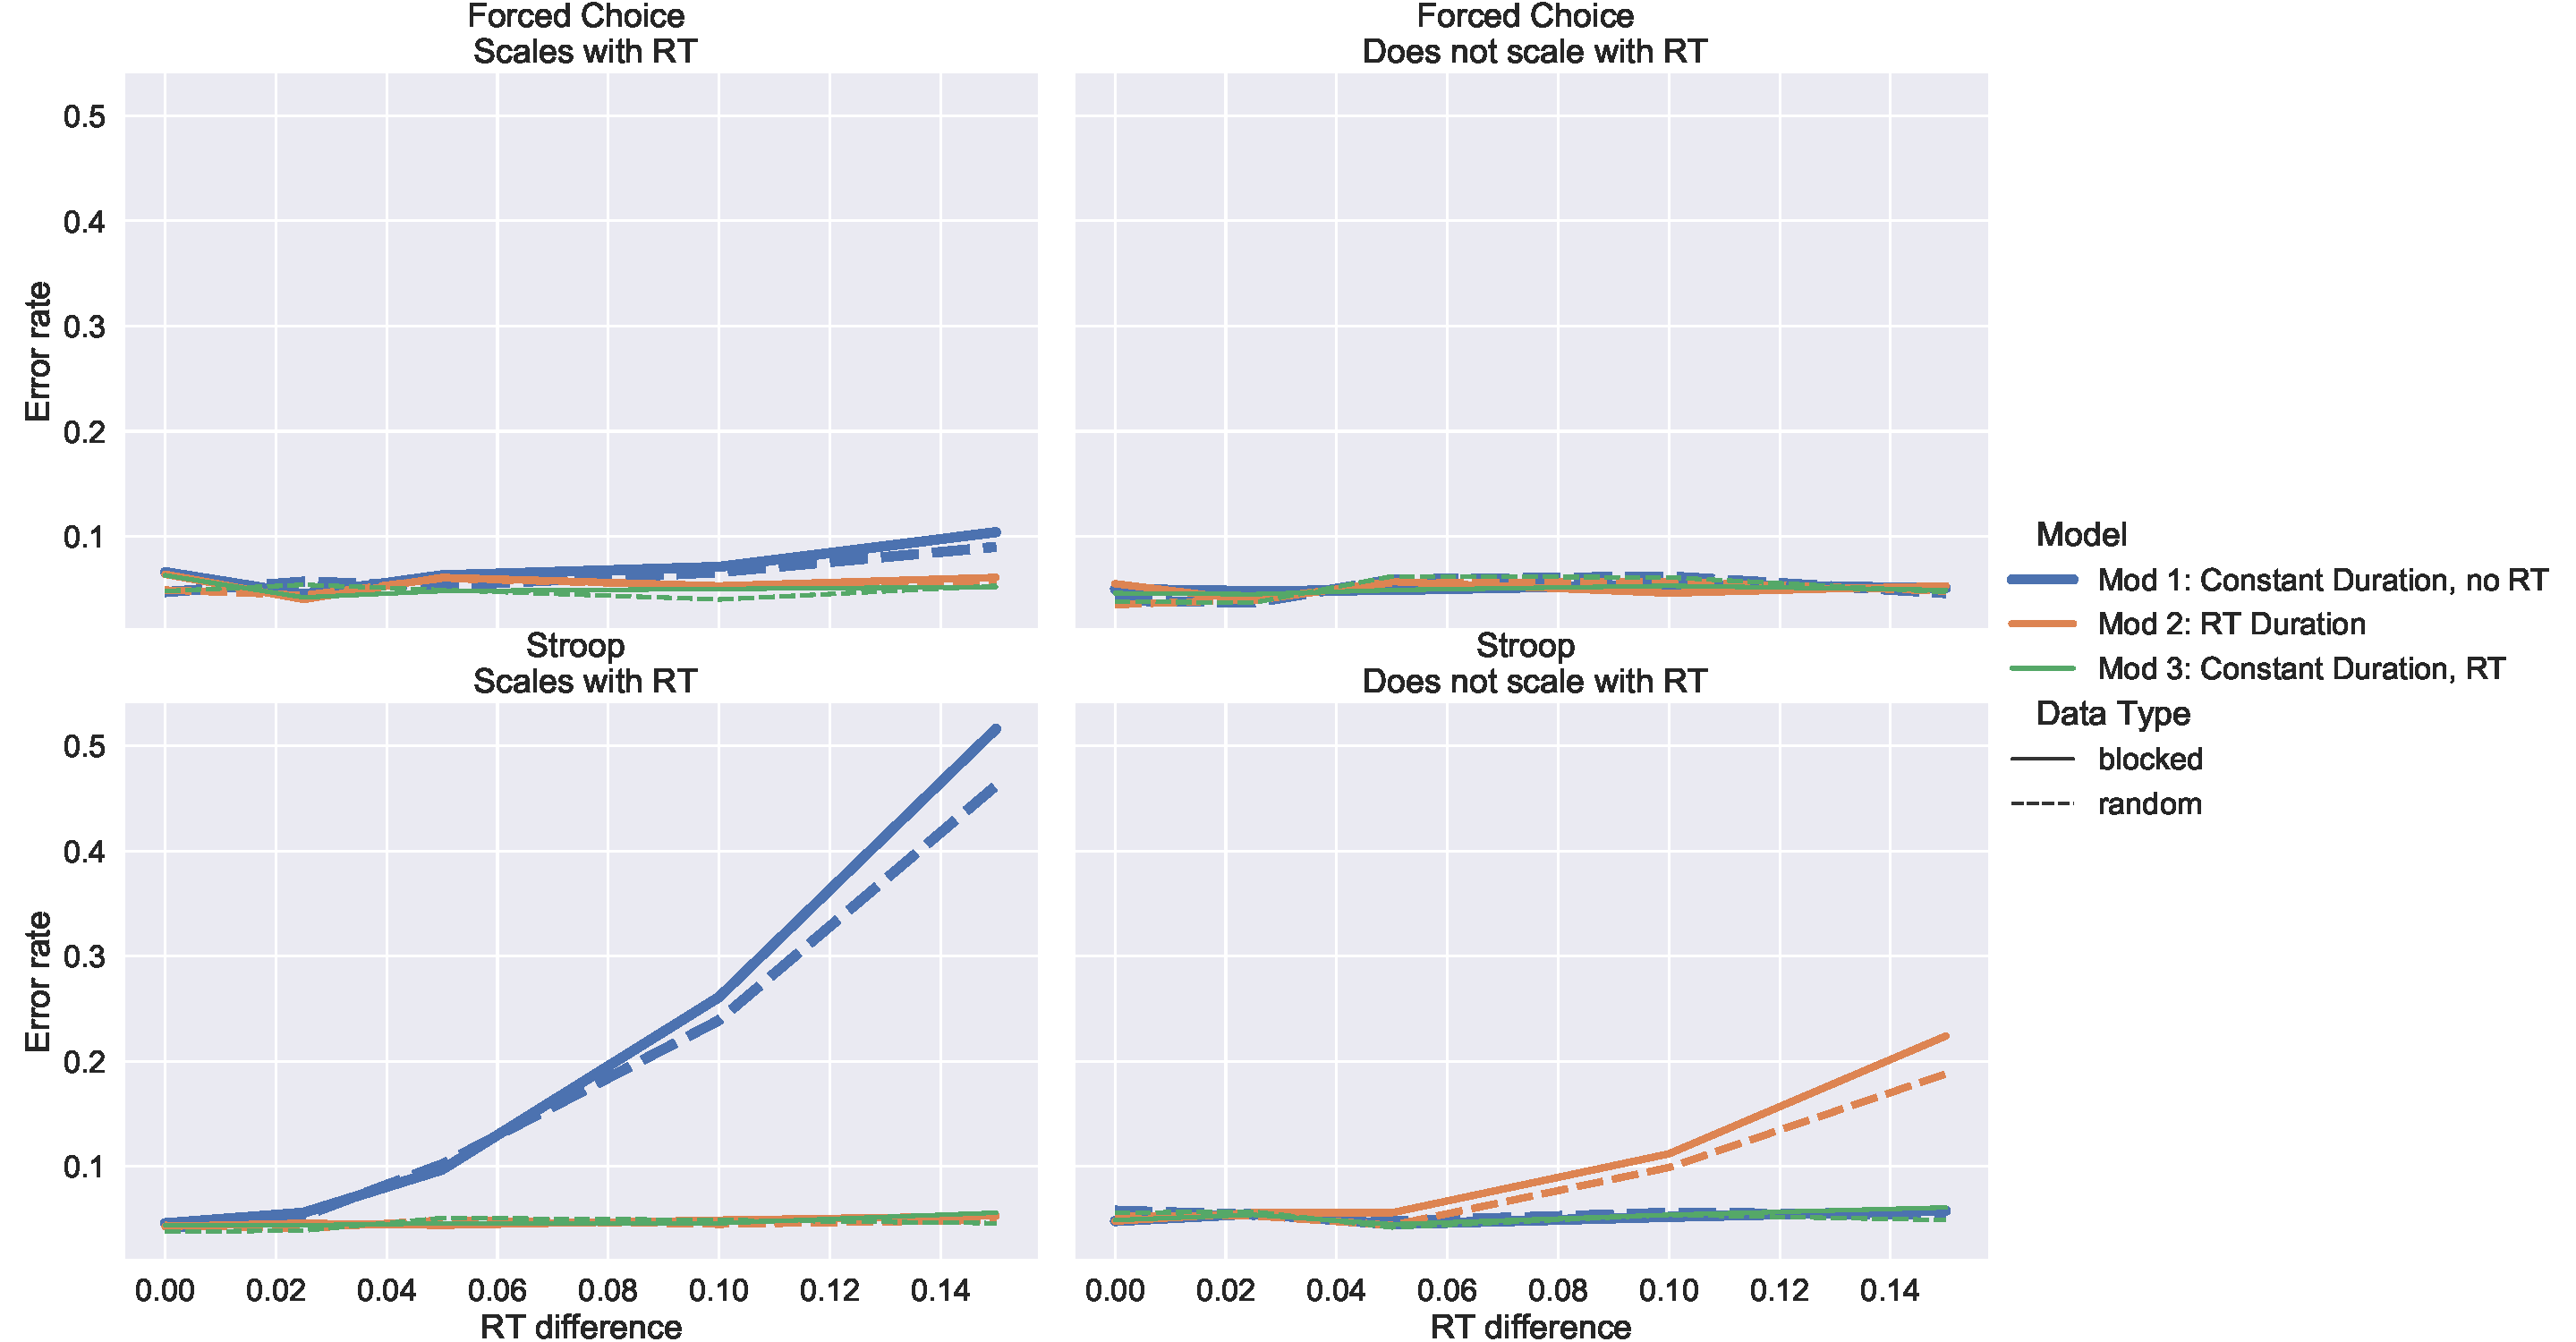
\includegraphics[width=5in]{Figures/type1_err_36.pdf}
   \caption{Type I error as RT difference between conditions increases.  This illustrates that results are similar to when the ISI ranged between 2-4s (result in main manuscript).  The Forced Choice Task RT distribution was used in the top panels, while Stroop RT distribution was used in the bottom panels, both with an ISI between 3-6s was used and inference of interest was the 1-sample t-test of the condition effect with 100 subjects.  2500 simulations were used to calculate the error rate.}
  \label{fig:type1err_36}
\end{figure}

\subsection*{Power differences when studying condition differences after testing for interaction}
Here we study the power for a condition effect after testing for a potential condition by RT interaction.  The interaction model contained two condition regressors and two RT regressors, split by condition. RTs were centered by the theoretical RT based on the distribution used to simulate RTs.  Although the slopes of the interaction model were not found to significantly differ, their magnitudes will not be exactly equal and this introduces variance into the condition difference estimate from this model.  This is reflected in the reduced power compared to the ConsDurRT model (Figure \ref{fig:pow-int}).
\begin{figure}[h!]
  \centering
   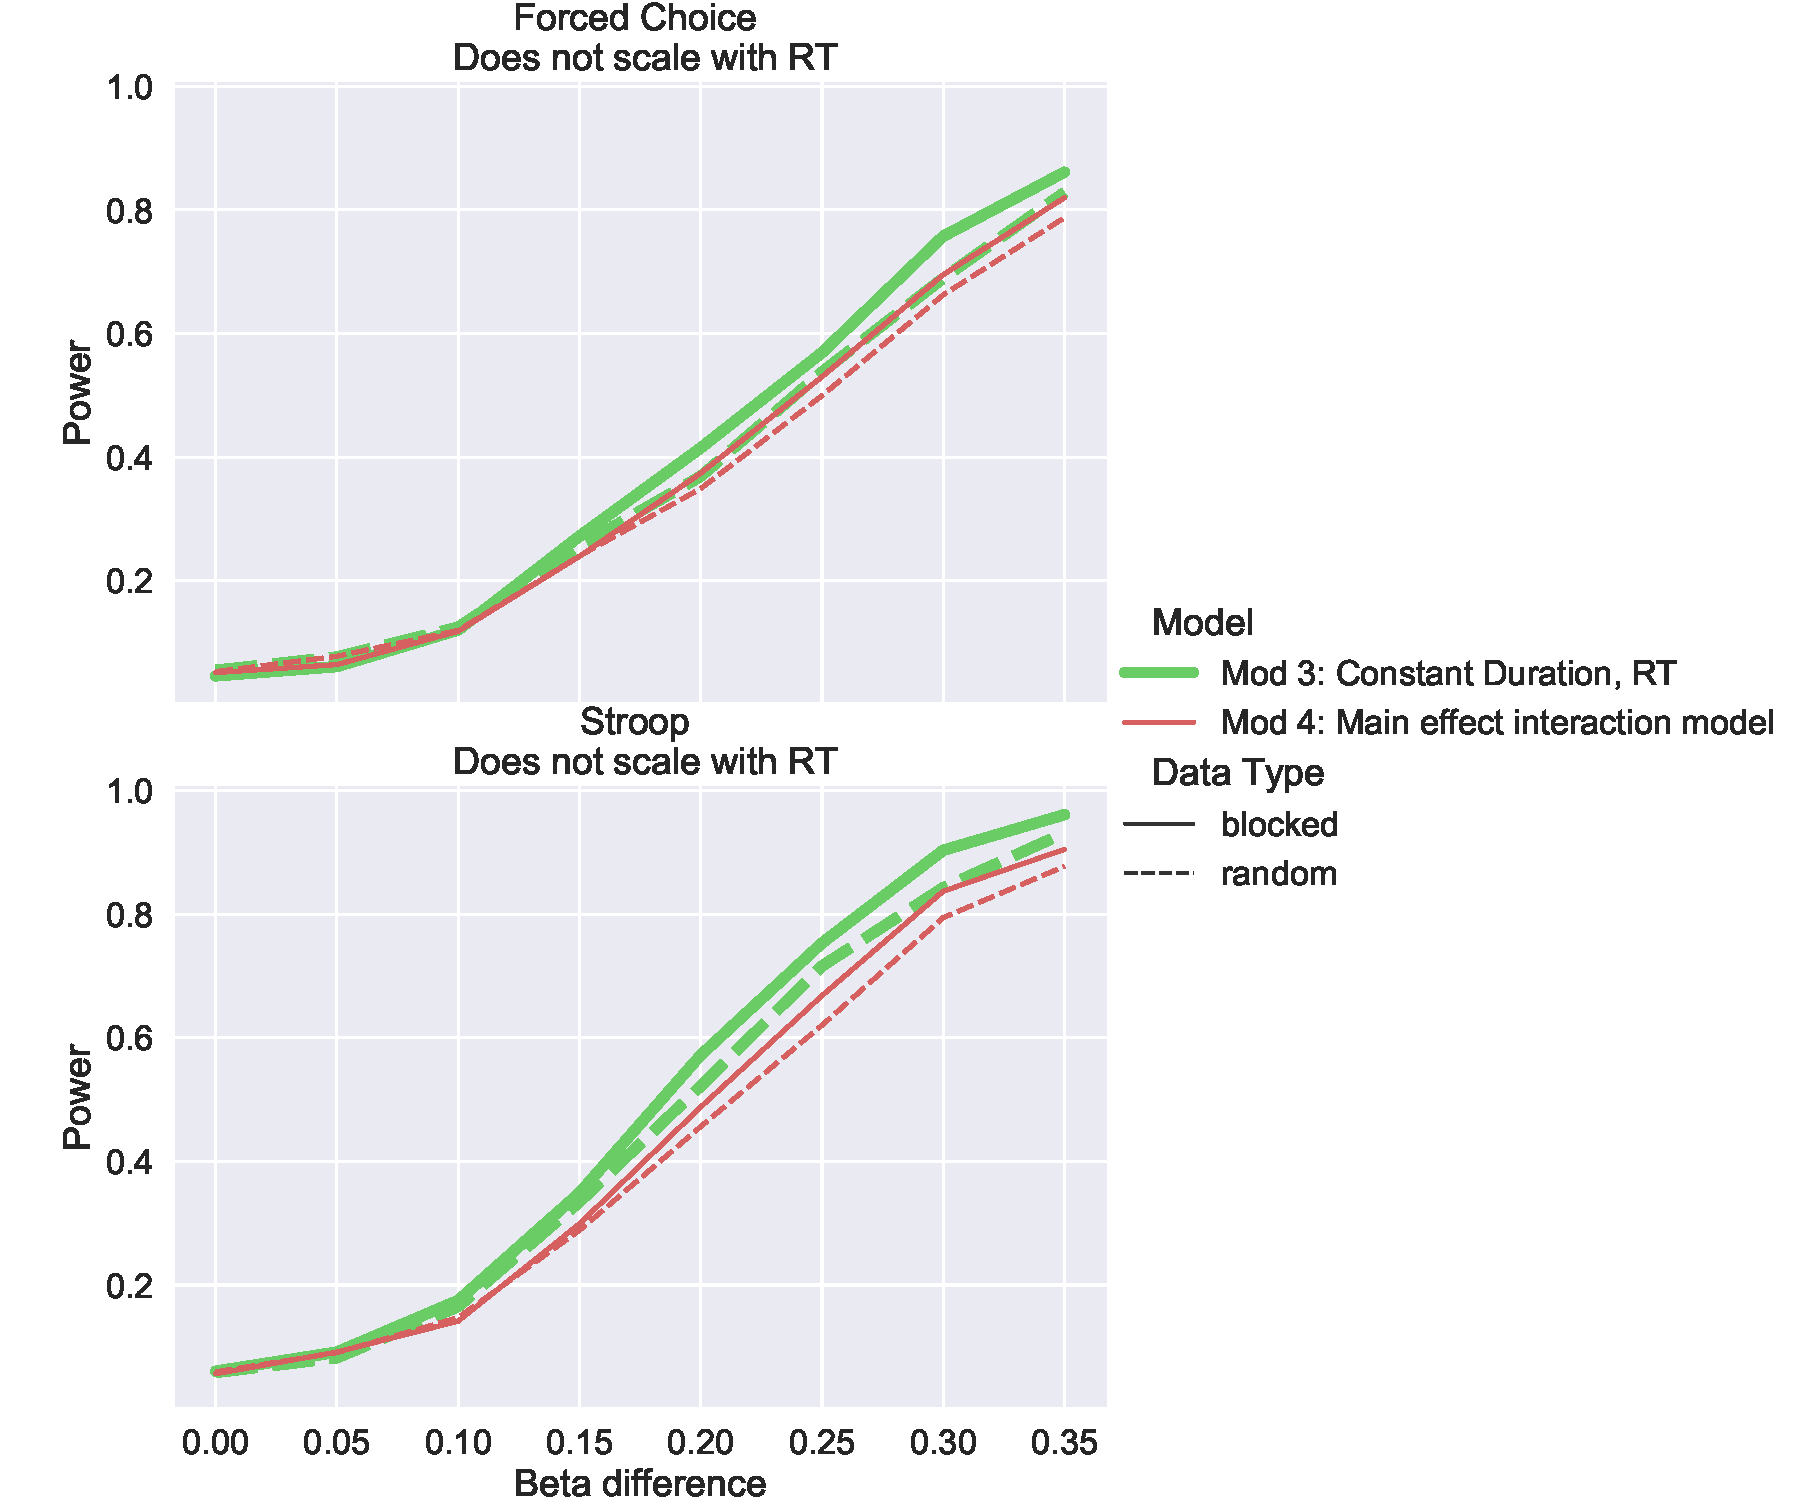
\includegraphics[width=5in]{Figures/power_24_rtdiff_1_interaction.pdf}
   \caption{Power for testing main condition difference effect after an interaction was found to be not significant.  Power is lost if the main effect of condition is studied in the interaction model, directly, due to the estimated sloped not being equal, which introduces variability into the estimate.  Power is improved if the condition difference is then studied using the ConsDurRT model.  Note, the p-value cutoff for testing the interaction and main effect of condition were set to .025 to preserve the overall error rate at 5\%.}
  \label{fig:pow-int}
\end{figure}



\newpage

\subsection*{Details about tasks involved in real data analysis}


The Attention Network Test (ANT) is a task designed to test three attentional networks: (1) alerting, (2) orienting, and (3) executive control. The ANT combines attentional and spatial cues with a flanker task (a central imperative stimulus is flanked by distractors that can indicate the same or opposite response to the imperative stimulus). On each trial a spatial cue is presented, followed by an array of five arrows presented at either the top or the bottom of the computer screen. The subject must indicate the direction of the central arrow in the array of five. The cue that precedes the arrows can be non-existent, a center cue, a double cue (one presented at each of the two possible target locations), or a spatial cue that deterministically indicates the upcoming target location. Each network is assessed via reaction times (RTs). The alerting network contrasts performance with and without cues, the orienting network contrasts performance on the task with or without a reliable spatial cue, and executive control (conflict) is measured by assessing interference from flankers.

The Dot Pattern Expectancy (DPX) task measures individual differences in cognitive control. Participants are presented with a cue made up of dots. This cue can be a valid cue – referred to as A (e.g., ":") – or an invalid cue – referred to as B (e.g., ".."). Next a probe is presented, also made up of a simple dot formation. This probe can be valid (X) or invalid (Y). Participants are instructed to respond to valid probe and cue combinations (targets – AX combinations) with a key press (e.g., “x”) and all others (non-targets) with a different key press (e.g., “m”).

The Delay-Discounting Task (DDT) is a measure of temporal discounting, the tendency for people to prefer smaller, immediate monetary rewards over larger, delayed rewards. Participants complete a series of 27 questions that each require choosing between a smaller, immediate reward (e.g., \$25 today) versus a larger, later reward (e.g., \$35 in 25 days). The 27 items are divided into three groups according to the size of the larger amount (small, medium, or large). Modeling techniques are used to fit the function that relates time to discounting. The main dependent measure of interest is the steepness of the discounting curve such that a more steeply declining curve represents a tendency to devalue rewards as they become more temporally remote.

The cued task-switching task indexes the control processes involved in reconfiguring the cognitive system to support a new stimulus-response mapping. In this task, subjects are presented with a task cue followed by a colored number (between 1-4 or 6-9). The cue indicates whether to respond based on parity (odd/even), magnitude (greater/less than 5), or color (orange/blue). Trials can present the same cue and task, or can switch the cue or the task. Responses are slower and less accurate when the cue or task differs across trials (i.e. a switch) compared to when the current cue or task remains the same (i.e. a repeat).

The Stop-Signal Task is designed to measure motor response inhibition, one aspect of cognitive control. On each trial of this task participants are instructed to make a speeded response to an imperative ``go'' stimulus except on a subset of trials when an additional ``stop signal'' occurs, in which case participants are instructed that they should make no response. The Independent Race Model describes performance in the Stop-Signal Task as a race between a go process that begins when the go stimulus occurs and a stop process that begins when the stop signal occurs. According to this model, whichever independent process reaches completion first determines the resulting behavior; earlier completion of the go process results in an overt response (i.e., stop-failure), whereas earlier completion of the stop process results in successful inhibition. The main dependent measure, stop-signal reaction time (SSRT), can be computed such that lower SSRT indicates greater response inhibition. One variant of the task measures proactive slowing, the tendency for participants to respond more slowly in anticipation of a potential stopping signal. This variant often uses multiple probabilities of a stop signal (e.g., 20\% and 40\%) to manipulate participants’ expectancies about the likelihood of a stop signal occurring. The extent of slowing in the higher compared to the lower stop probability conditions is an index of proactive slowing/control.

The motor selective stop-signal task measures the ability to engage response inhibition selectively to specific responses. In this task, cues are presented to elicit motor responses (e.g., right hand responses, left hand responses). A stop-signal is presented on some trials, and subjects must stop if certain responses are required on that trial (e.g., right hand responses) but not others (e.g., left hand responses) if a signal occurs. In contrast to a simple stop-signal task in which all actions are stopped when a stop-signal is presented, this task aims to be more like stopping in ``the real world'' in that certain motor actions must be stopped (e.g., stop pressing the accelerator at a red light) but others should proceed (e.g., steering the car and/or conversing with a passenger). Commonly, stop-signal reaction time (SSRT), the main dependent measure for response inhibition in stopping tasks, is prolonged in the motor selective stopping task when compared to the more canonical simple stopping task. This prolongation of SSRT is taken as evidence of the cost of engaging inhibition that is selective to specific effectors or responses.

The Stroop task is a seminal measure of cognitive control. Successful performance of the task requires the ability to overcome automatic tendencies to respond in accordance with current goals. On each trial of the task, a color word (e.g., ``red'', ``blue'') is presented in one of multiple ink colors (e.g., blue, red). Participants are instructed to respond based upon the ink color of the word, not the identity of the word itself. When the color and the word are congruent (e.g., “red” in red ink), the natural tendency to read the word facilitates performance, resulting in fast and accurate responding. When the color and the word are incongruent (e.g., ``red'' in blue ink), the strong, natural tendency to read must be overcome to respond to the ink color. The main dependent measure in the Stroop task is the ``Stroop Effect'', which is the degree of slowing and the reduction in accuracy for incongruent relative to congruent trials.




\end{document}

